\documentclass[main.tex]{subfiles}

\begin{document}

\section{Parton showers in vacuum}
Beginning, we will limit ourselves to generating jets consisting exclusively of gluons in a vacuum.

\subsection{Evolution interval }\label{sec: determining_evolution_time_from_sudakov}
The Jets will evolve according to the evolution variable given in \autoref{eqn: evolution_parameter_dasguptalike}. With the fixed coupling, and integrating it rewrites as, 
\begin{align}\label{eqn: evolution_parameter_integrated}
    t &= \frac{\alpha_S}{2\pi} ln(\frac{R^2}{\theta^2})
\end{align}
Now we need to determine the limits of this evolution variable. If we disregard the distributions from the DGLAP equation, and consider it a splitting probability function on the form,
\begin{equation}\label{eqn: dglap_ellis_style_probability_thetafunc}
    P_{tot} = \int_0^1 \frac{dz}{z} \int_0^{t} \frac{dt}{t} \, P(z) \, \Theta(k_\perp >Q_0)
\end{equation}
where \(\Theta(k_\perp >Q_0)\) serves to show that splittings may only occur down to the hadronization scale \(Q_0\). It can be absorbed into the integration limits by starting with the criteria, \textcolor{red}{ criteria comes from where? }
\begin{align}
    \begin{split}
        k_\perp &= z(1-z)\, p_t\, \theta > Q_0  \\
        k_\perp &\approx z\, p_t\, \theta > Q_0 \textcolor{red}{???}
    \end{split}
\end{align}
it can be shown that the constraint on z is,
\begin{align}
    1 > z &> \frac{4\cdot Q_0}{p_t\, \theta}
\end{align}
and the constraints on \(\theta\) is similarly,
\begin{equation}
     R>\theta >\frac{Q_0}{z(1-z)\, p_t} %>\frac{4 Q_0}{p_t} >\frac{ Q_0}{p_t}
\end{equation}
Since the Monte-Carlo will be imposing the limits on \(t \sim ln(1/\theta^2) \), before picking a parton to split, it will be convenient to write the limits of \(\theta\) independently of \(z\) by making the following replacement,
\begin{align}
    R>\theta &>\frac{Q_0}{z(1-z)\, p_t} > \frac{Q_0}{\frac{Q_0}{p_t \, R}(1-\frac{Q_0}{p_t \, R})\, p_t} \nonumber\\
    R>\theta &>\frac{1}{\frac{1}{R} (1-\frac{Q_0}{p_t \, R})} \nonumber\\
    R>\theta &>\frac{R}{1 - \frac{Q_0}{p_t R}} \label{eqn: DGLAP_limits_zandtheta}
\end{align}
Now all that remains is to write the limits in terms of t, instead of \(\theta\). From \autoref{eqn: evolution_parameter_integrated} we find, 
\begin{align}
    t\cdot \frac{2\pi}{\alpha_S} &= ln\left(\frac{R^2}{\theta^2} \right) \nonumber \\
    \exp \left(t\cdot \frac{2\pi}{\alpha_S} \right) &= \frac{R^2}{\theta^2} \nonumber \\
    \theta^2 &= R^2 \cdot \exp \left(- t\cdot \frac{2\pi}{\alpha_S} \right) \nonumber \\
    \theta &= R \cdot \sqrt{\exp\left(-t\cdot \frac{2\pi}{\alpha_S}\right)}
\end{align}
we can then determine the limits by inserting this expression for \(\theta\) into \autoref{eqn: DGLAP_limits_zandtheta}, 
\begin{align}
    R> R \cdot \sqrt{\exp\left(-t\cdot \frac{2\pi}{\alpha_S}\right)} &>\frac{R}{1 - \frac{Q_0}{p_t R}} \nonumber \\
    1> \exp\left(-t\cdot \frac{2\pi}{\alpha_S}\right) &> \left(\frac{1}{1 - \frac{Q_0}{p_t R}}\right)^2 \nonumber \\
    \ln(1)> \left(-t\cdot \frac{2\pi}{\alpha_S}\right) &> \ln(\frac{1}{1 - \frac{Q_0}{p_t R}})^2 \nonumber \\
     0< \left(t\cdot \frac{\pi}{\alpha_S}\right) &< \ln(\frac{1}{1 - \frac{Q_0}{p_t R}}) 
\end{align}
and the limits on our evolution variable is therefore, 
\begin{equation}\label{eqn: evolution_parameter_boundaries}
    \frac{\alpha_S}{\pi} \ln(\frac{1}{1 - \frac{Q_0}{p_t R}}) > t > 0
\end{equation}
\autoref{fig: evolution_variable_vacuumshowers} is a plot of the maximum value of \(t\) for a range of values for \(R\) and \(p_t\). 
\begin{figure}[h]
    \centering
    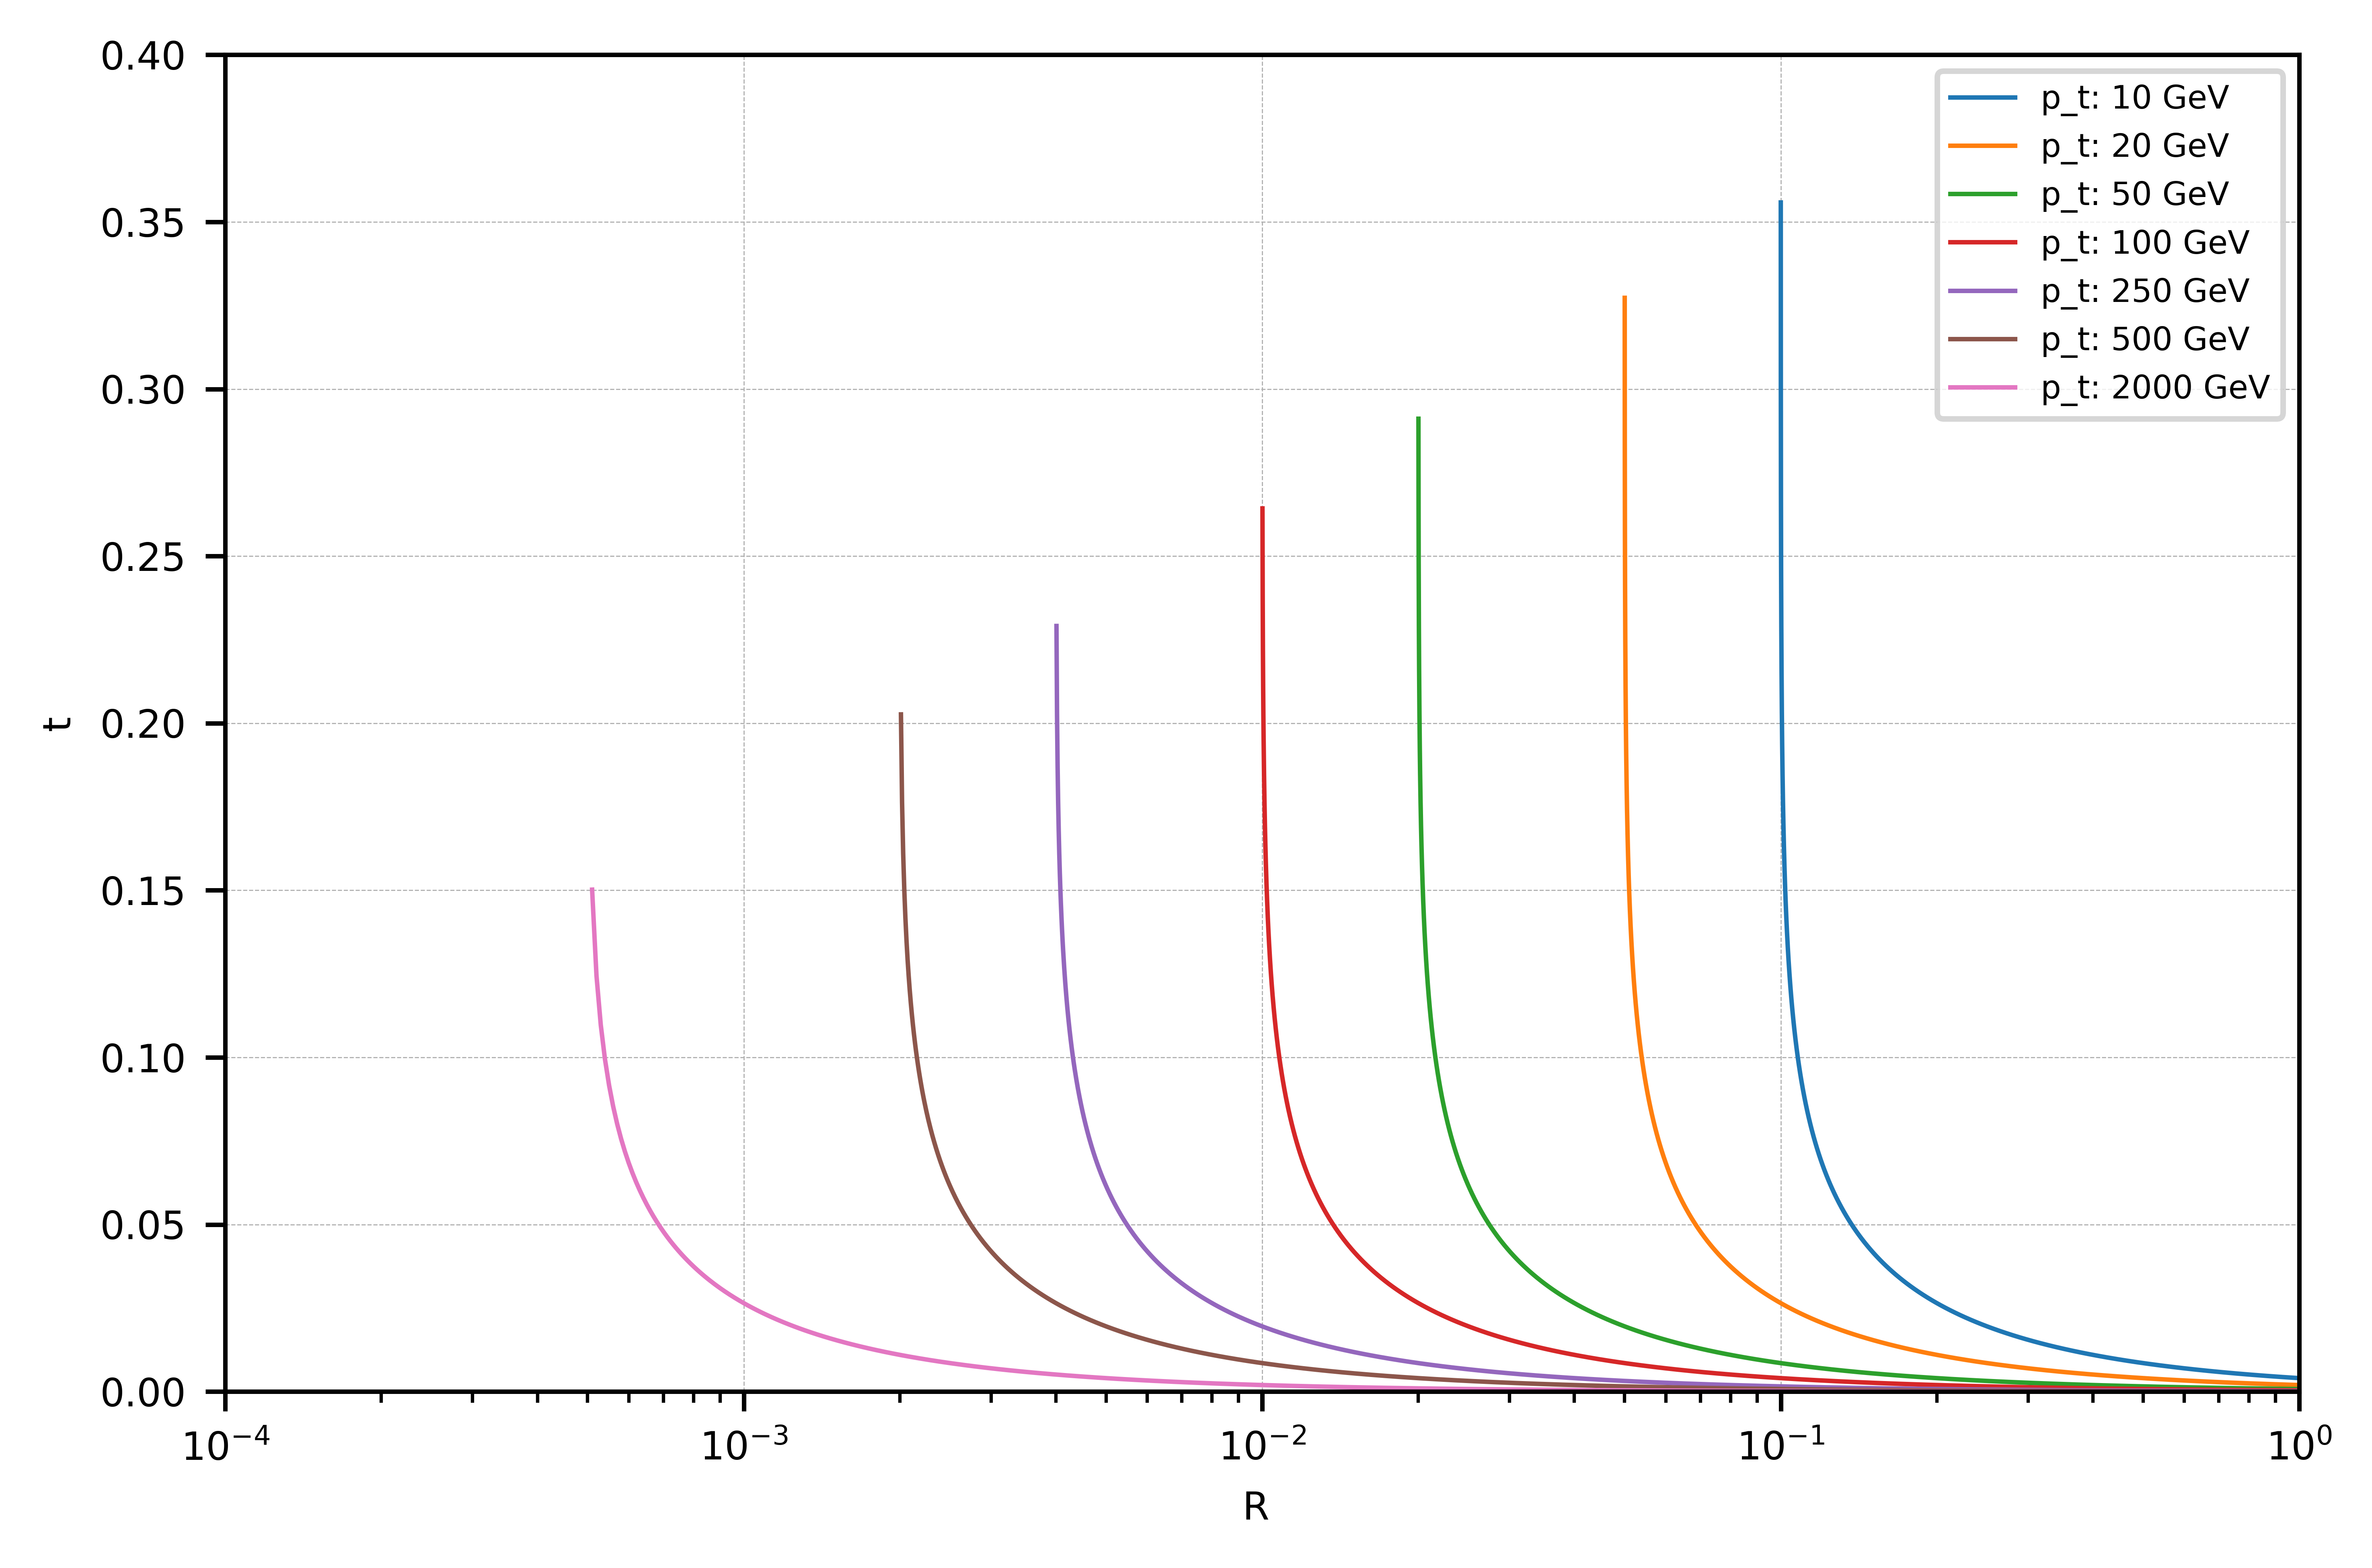
\includegraphics[width=10cm]{pictures/misc/evolution_variable_vacuumshowers.png}
    \caption{Evolution variable for vacuum showers, plotted up to \(p_t\cdot R > Q_0\). Here \(\alpha_S = 0.12\).}
    \label{fig: evolution_variable_vacuumshowers}
\end{figure}
Knowing the boundaries we need to impose on the evolution parameter for our MC, we can now move on to determining how to sample intervals of the evolution parameter.
This can be done using the Sudakov form factor - which is related to the branching probability - to randomly determine an interval \(\Delta t\) in which we can expect a branching. This is because the probability of \textit{no} branching in the interval \([t_0, t]\), is given directly from the Sudakov form factor,
\begin{equation}\label{eqn: branching_probability_from_sudakov}
    \mathcal{P}(\Delta t) = \frac{\Delta(t)}{\Delta(t_0)} = exp\left(-\Delta t \int_\epsilon^{1-\epsilon}dz \, p_{gg}(z)\right) 
\end{equation}
Therefore, we can generate a random number in the interval \(\mathcal{P}(\Delta t) = \mathcal{R} \in [0,1]\), and use it to solve for \(\Delta t\), at which we can expect to get a new splitting, 
%\begin{equation*}
%    \mathcal{R} = exp\left(-\Delta t \int_\epsilon^{1-\epsilon}dz \, p_{gg}(z)\right) 
%\end{equation*}
\begin{equation}\label{eqn: expected_branching_interval}
    \Delta t = -\frac{ln(\mathcal{R})}{ \int_\epsilon^{1-\epsilon}dz \, p_{gg}(z)} 
\end{equation}
Therefore, in our Monte Carlo, the evolution boundaries will be implemented as follows, 
\begin{enumerate}
    \item Calculate the maximum angle \(t_{\text{max}}\) as given from \autoref{eqn: evolution_parameter_boundaries}.
    \item Calculate the expected interval \(\Delta t\) for a branching according to \autoref{eqn: expected_branching_interval}.
    \item Evolve the angle \(t\) by \(\Delta t\).
    \item Continue as long as \(t< t_{\text{max}}\). 
\end{enumerate}
\subsection{Managing quarks and gluons}\label{sec: managing_quarks_and_gluons}
When creating a program with both quarks and gluons, we need to evolve the interval based on which kind of parton we are splitting. When splitting a quark the inteval will evolve according to \autoref{eqn: sudakov_splitting_interval_quarks}, and when splitting a gluon it will evolve according to \autoref{eqn: sudakov_splitting_interval_gluons}.
\begin{align}
    \mathcal{P}_{q}(\Delta t) &= exp\left(-\Delta t \int_\epsilon^{1-\epsilon} p_{qq}(z) \, dz \right) \label{eqn: sudakov_splitting_interval_quarks}\\
    \mathcal{P}_{g}(\Delta t) &= exp\left(-\Delta t \int_\epsilon^{1-\epsilon} p_{gq}(z) + p_{gg}(z) \, dz \right)  \label{eqn: sudakov_splitting_interval_gluons}  
\end{align}
The question that remains is how to determine what parton to branch. Assuming the available interval \(t\) is large enough for either splitting to occur, and that there are available partons of both kinds, then we need to determine the contributions of each parton to the full Sudoku form-factor given by \autoref{eqn: full_sudakov_splitting_interval_gluons&quarks},
\begin{equation}\label{eqn: full_sudakov_splitting_interval_gluons&quarks} 
    \mathcal{P}_{\text{full}}(\Delta t) = exp\left(-\Delta t \int_\epsilon^{1-\epsilon}( p_{qq}(z) + p_{gq}(z) + p_{gg}(z) )\, dz \right) 
\end{equation}
From this the contributions \(W_{q,g}\) from the quarks and gluons are respectively, 
\begin{equation}\label{eqn: parton_selection_ratios}
    W_q = \frac{\mathcal{P}_{q}(\Delta t)}{\mathcal{P}_{\text{full}}(\Delta t)} \qquad , \quad 
    W_g = \frac{\mathcal{P}_{g}(\Delta t)}{\mathcal{P}_{\text{full}}(\Delta t)}
\end{equation}
Generally these ratios will be \(W_g > W_q\), meaning it is more probably to split a gluon than a quark. Therefore when deciding on which kind of parton to split we will throw a random number \(\mathcal{R}\), and if \(\mathcal{R} < W_g\) we will split a gluon, and if \(\mathcal{R} \geq W_g\) we will split a quark.

Similarly, when deciding weather to split a gluon using the \ggg or \gqq splitting functions,
\begin{equation}\label{eqn: gluon_splitting_selection_ratios}
    W_{ggg} = \frac{\int_\epsilon^{1-\epsilon} p_{gg}(z) \, dz}{\int_\epsilon^{1-\epsilon}p_{gq}(z) + p_{gg}(z) \, dz}
\end{equation}

\subsection{Sampling random energy fractions from the splitting functions}\label{sec: metropolis_hastings}
Now, that we know at what evolution interval we can expect to get a branching and how to select quarks or gluons to branch, we must determine the momentum fraction carried by the branched partons.
This can be done if we consider the probability density given as,
\begin{equation}\label{eqn: probability_density_for_splitting}
    \mathcal{P}(z) = \frac{ p_{gg}(z)}{\int_\epsilon^{1-\epsilon} dz \, p_{gg}(z)}
\end{equation}
which means that we can generate random momentum fractions for the branched parton, to be equal the distribution of \eqref{eqn: probability_density_for_splitting}, by the following relation,
\begin{equation}\label{eqn: energyfraction_function_R}
    \mathcal{R} \cdot \int_\epsilon^{1-\epsilon} dz \, p_{gg}(z) = \int_\epsilon^{y}dz \, p_{gg}(z)
\end{equation}
where \(\mathcal{R}\in [0,1]\), equivalent to equation (5.60) of Ellis \cite{ellis_stirling_webber_1996}.

When trying to solve \autoref{eqn: energyfraction_function_R} for the different splitting functions, we will find that not all of them can be solved for a general momentum-fraction \(y\), and we need to introduce the Metropolis-Hastings algorithm \cite{enwiki:1048445594}, for sampling them correctly.

For this algorithm we need the following,
\begin{itemize}
    \item A target distribution \(P(x)\), which is the one we are trying to sample.
    \item A proposal distribution \(f(x)\) proportional to \(\mathcal{P}(x)\).
\end{itemize}
The Metropolis-Hastings algorithm will then be implemented as follows:
\begin{enumerate}
    \item We start by sampling a random value \(x'\) from our proposal distribution \(P(x)\).
    \item Now we need to calculate the acceptance probability,
    \[A(x') = \text{min} \left(1, \, \frac{P(x')}{f(x')}\right)\]
    \item Next we need to decide if we will accept or reject the new state,
    \begin{enumerate}[i)]
        \item Generate a random number \(\mathcal{R}\in [0,1]\).
        \item If \(u\leq A(x')\), then accept the new value, and continue.
        \item Else, we reject the new value, and start over from step 2.
    \end{enumerate}
\end{enumerate}

We will now use \autoref{eqn: energyfraction_function_R} to sample random energy fractions, proportionally to the full splitting functions as derived in \autoref{sec: derivation_splitting_functions_vacuum}.

\subsubsection{Sampling from the ggg vertex in vacuum}
When trying to solve \autoref{eqn: energyfraction_function_R} for the \ggg splitting function in \autoref{eqn: vacuum_ggg_splitting_function}, we will see that it is difficult to solve for \(y\). We will therefore introduce a simplified splitting function, which can be used in the Metropolis-Hastings algorithm.
\begin{equation}\label{eqn: p_ggg_vacuum_dummy}
    p^{\text{(dummy)}}_{gg}(z) = \frac{1}{z(1-z)}
\end{equation}
the integral of this function can generally be shown to be, 
\begin{align}
    \int_a^b \frac{1}{z(1-z)}dz &= \int_a^b \frac{1}{z}dz + \int_a^b \frac{1}{(1-z)}dz \nonumber\\
    &= \left[ ln (z)\right]_a^b - \left[ln(1-z) \right]_a^b  \nonumber\\
    &= ln (\frac{b}{a}) + ln(\frac{1-a}{1-b})
\end{align}
which means that we can evaluate \autoref{eqn: energyfraction_function_R} as,
\begin{align}
    \mathcal{R} \int_\epsilon^{1-\epsilon} dz \, \frac{1}{z(1-z)} &= \int_\epsilon^{y} \frac{1}{z(1-z)}  \nonumber\\
    \mathcal{R} \left(  ln (\frac{1-\epsilon}{\epsilon}) + ln(\frac{1-\epsilon}{\epsilon}) \right) &= ln (\frac{y}{1-y}) + ln(\frac{1-\epsilon}{\epsilon}) \nonumber\\
    \mathcal{R} \cdot 2 \left( ln (\frac{1-\epsilon}{\epsilon}) \right) &= ln (\frac{y}{1-y} \cdot \frac{1-\epsilon}{\epsilon})
\end{align}
exponentiating both sides, 
\begin{align}\label{eqn: MC_energyfraction_origin_vacuum}
    \frac{y}{1-y} \frac{1-\epsilon}{\epsilon} &= \left(\frac{1-\epsilon}{\epsilon}\right)^{2\cdot \mathcal{R}} \nonumber\\
    \frac{y}{1-y} &= \left(\frac{1-\epsilon}{\epsilon}\right)^{(2\cdot \mathcal{R}-1)} \nonumber\\
    y &= \frac{\left(\frac{1-\epsilon}{\epsilon}\right)^{(2\cdot \mathcal{R}-1)}}{1+\left(\frac{1-\epsilon}{\epsilon}\right)^{(2\cdot \mathcal{R}-1)}}
\end{align}
simplifying the expression we obtain \autoref{eqn: MC_energyfraction} which can be used to randomly generate parton energy fractions, 
\begin{equation}\label{eqn: MC_energyfraction}
    y(\mathcal{R}) = \frac{\xi}{1+ \xi} \qquad \text{for, } \quad \xi = \left(\frac{1-\epsilon}{\epsilon}\right)^{(2\cdot \mathcal{R}-1)}
\end{equation}

\begin{figure}[h]
    \centering
    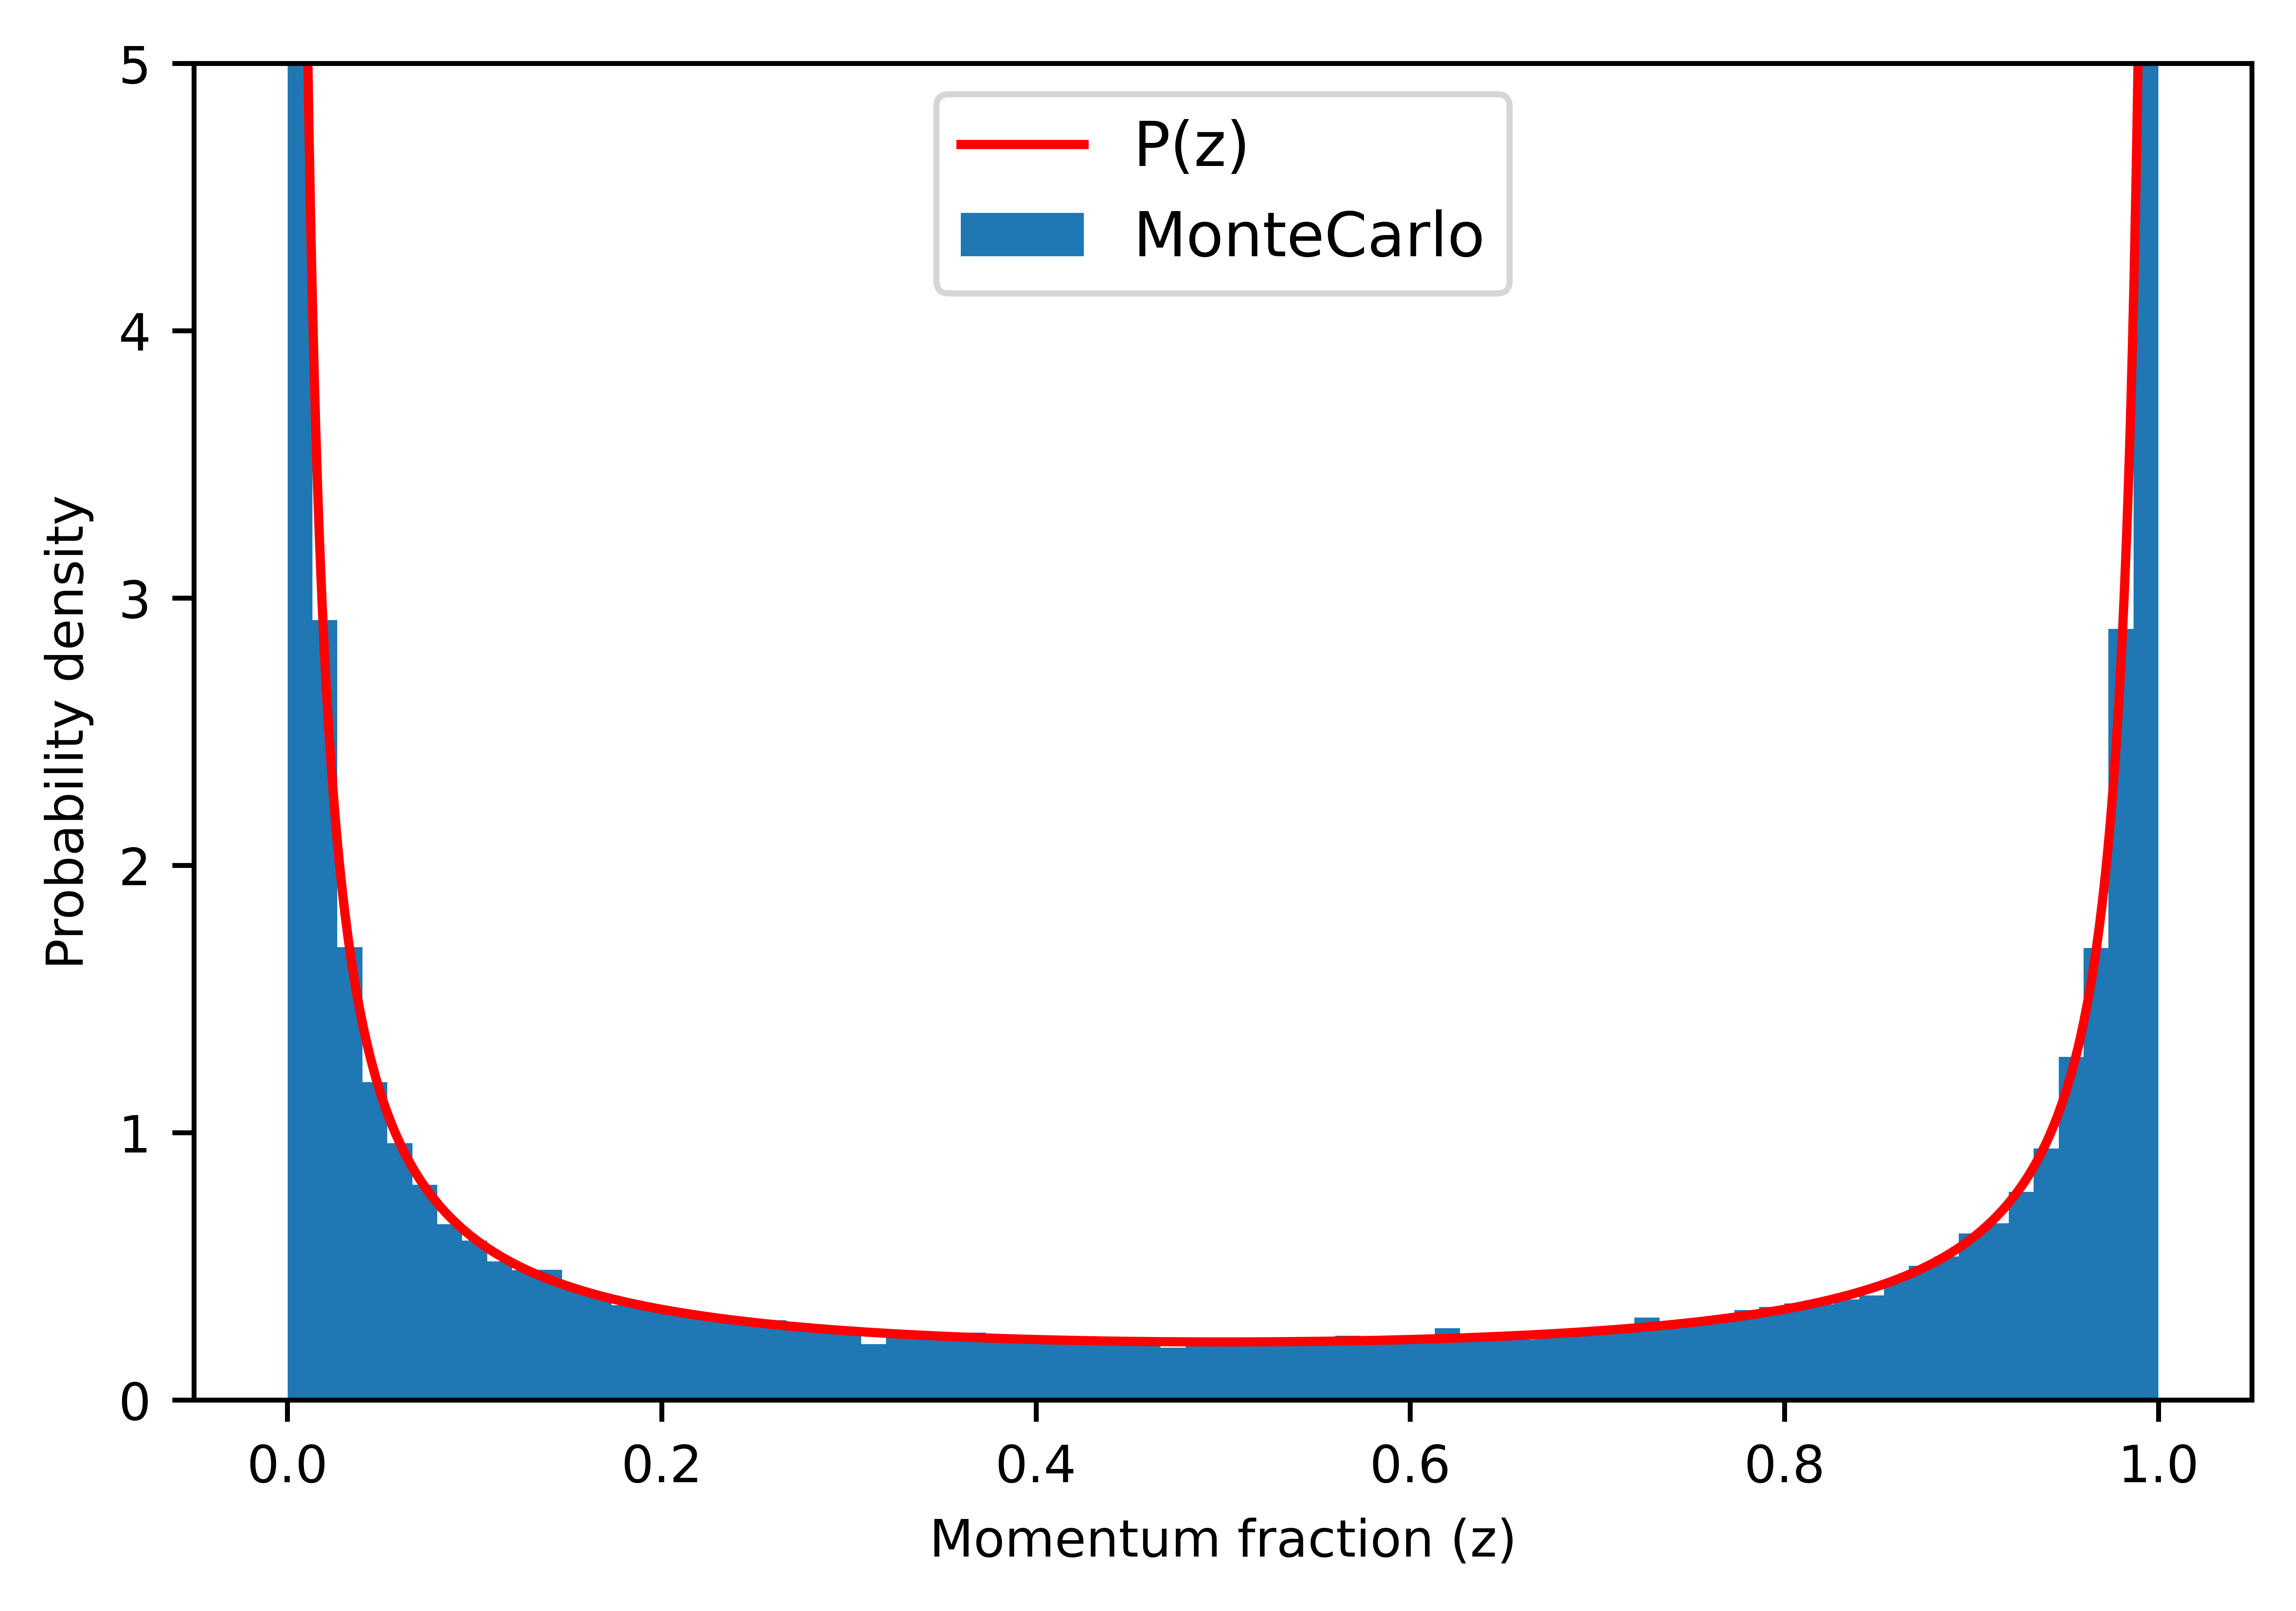
\includegraphics[width=7cm]{pictures/MH_plots/p_ggg_simple_MCvsPZ.png}
    \caption{Probability density for momentum fractions vs density histogram of randomly generated momentum fractions for a simplified \(p_{gg}\) splitting function. Generated with \(100,000\) points.\textcolor{red}{remove this}}
    \label{fig: function_vs_MC_simplified_pgg_splitting}
\end{figure}
\autoref{fig: function_vs_MC_simplified_pgg_splitting} gives the histogram of the sampled dummy splitting function values, compared to the exact dummy splitting function \autoref{eqn: p_ggg_vacuum_dummy}. 

\begin{figure}[h]
    \centering
    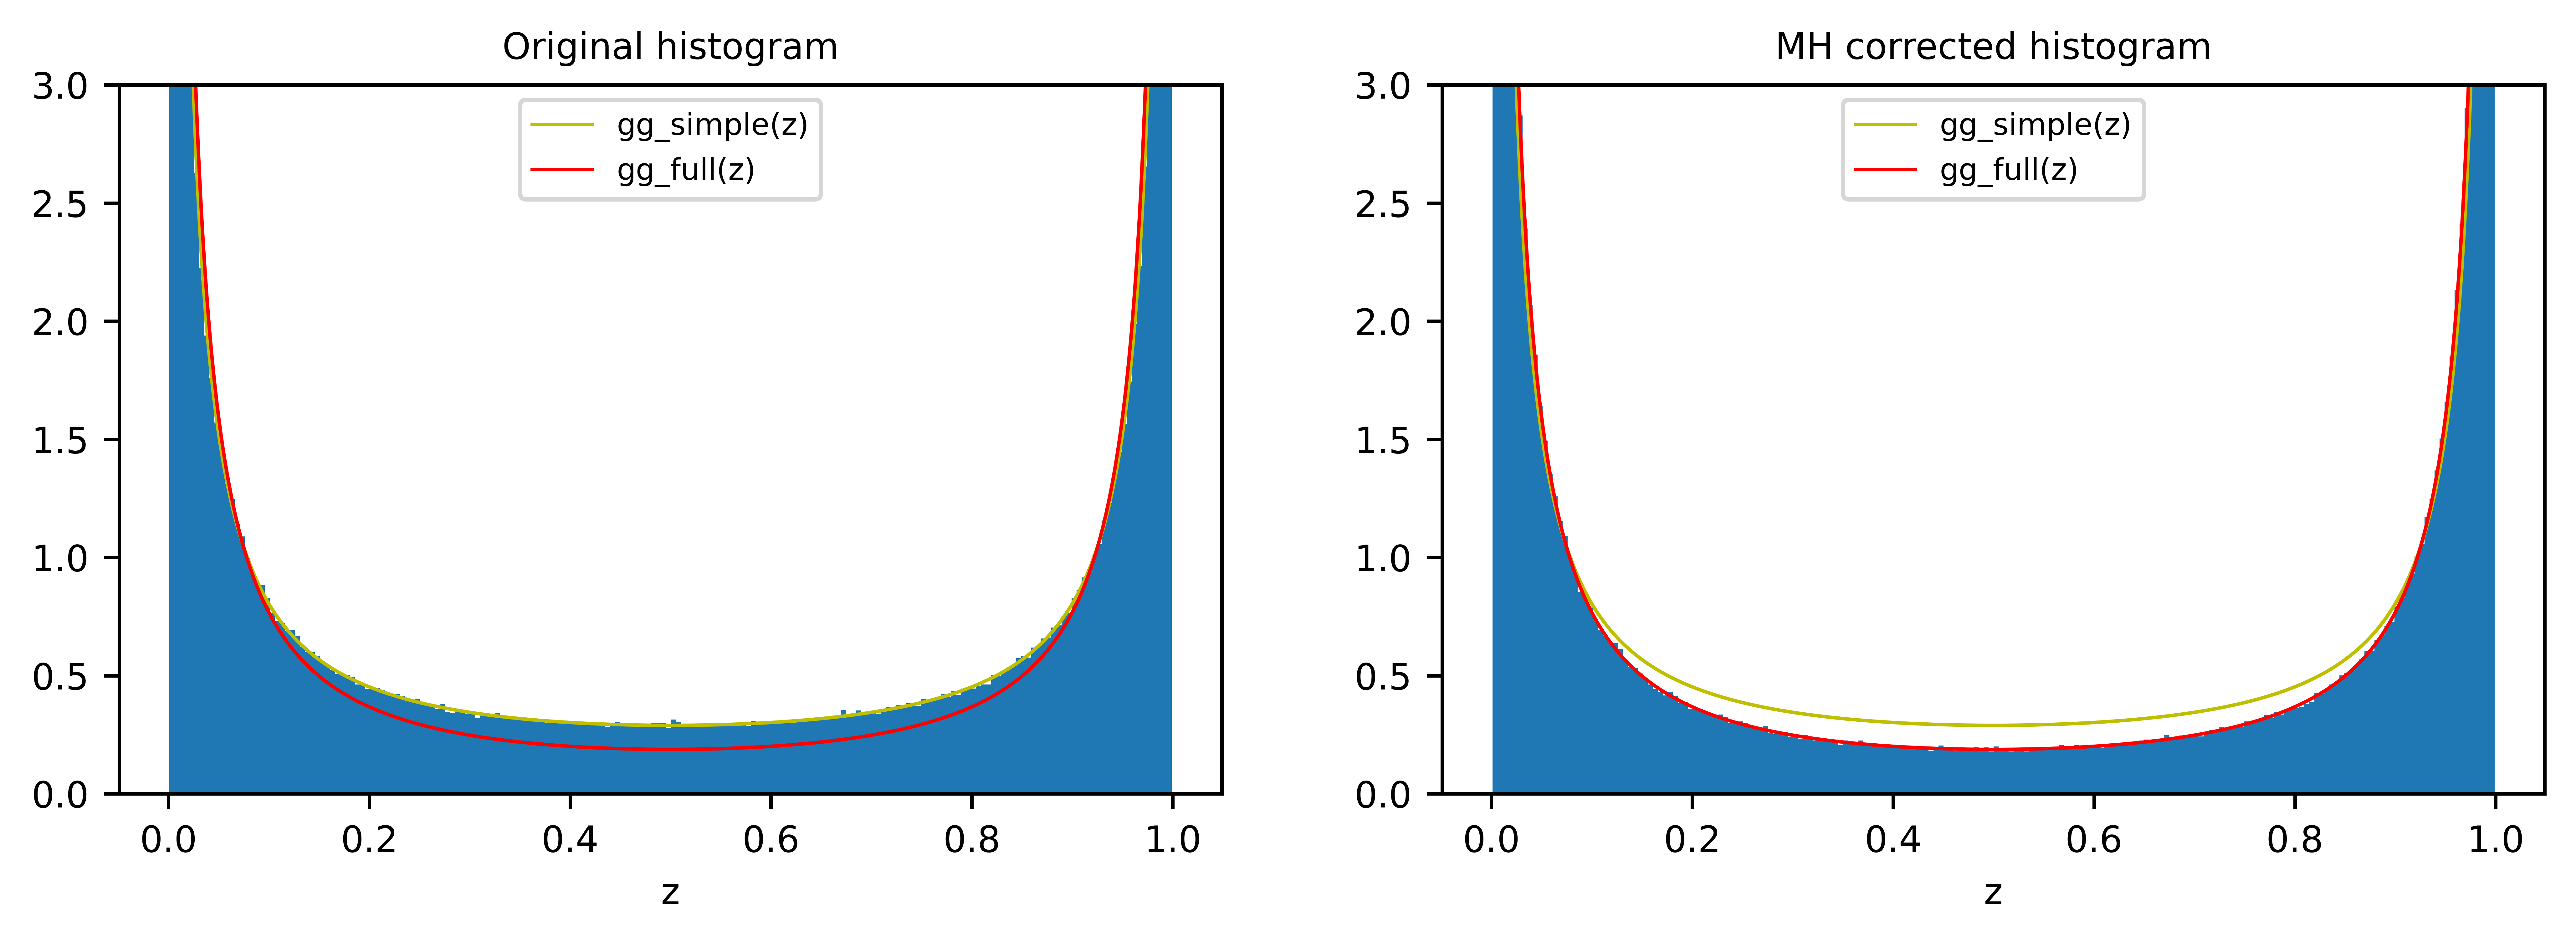
\includegraphics[width=14cm]{pictures/MH_plots/MH_vacuum_gg.png}
    \caption{Probability density of the full \(p_{gg}\) splitting function, compared to the density histogram of the dummy splitting function, and the Metropolis-Hastings corrected results. Simulated with \(1,000,000\) points, and an acceptance rate of \(0.87\).}
    \label{fig: MH_corrected_p_gg_splitting}
\end{figure}
\autoref{fig: MH_corrected_p_gg_splitting} gives us the results from the Metropolis-Hastings algorithm, when we are plotting the exact splitting function, and the histogram for our Monte-Carlo generated parton energy fractions determined by \autoref{eqn: MC_energyfraction}, and the Metropolis-Hastings corrected histogram.

\subsubsection{Sampling from the gqq vertex in vacuum}
Now we will try to solve \autoref{eqn: energyfraction_function_R} for the \gqq splitting function from \autoref{eqn: vacuum_gqq_splitting_function}. 
\begin{equation}\tag{\ref{eqn: energyfraction_function_R}}
    \mathcal{R} \cdot \int_\epsilon^{1-\epsilon} dz \, p_{gg}(z) = \int_\epsilon^{y}dz \, p_{gg}(z)
\end{equation}
The integral is, 
\begin{equation}
    \int_a^b dz\hat{P}_{qg}(z) = \int_a^b \left(z^2 + (1-z)^2 \right) = \int_a^b \left(1-2z+2z^2 \right) = \left[ z - z^2 + \frac{2}{3} z^3 \right]_a^b
\end{equation}
so by \(\epsilon = 10^{-3}\) \autoref{eqn: energyfraction_function_R} can be rewritten as,
\begin{align}
    \mathcal{R} \cdot \left[ z - z^2 + \frac{2}{3} z^3 \right]_\epsilon^{1-\epsilon} &= \left[ z - z^2 + \frac{2}{3} z^3 \right]_\epsilon^{y} \nonumber\\
    \mathcal{R} \cdot 0.665 &= (y - y^2 + \frac{2}{3} y^3) - 0.001 \\
\end{align}
We then end up with a cubic formula, 
\begin{equation}\label{eqn: gqq_vertex_qubic_formula}
    \frac{2}{3} y^3 - y^2 + y - (\mathcal{R} \cdot 0.665+0.001) = 0
\end{equation}
setting \(d = (\mathcal{R} \cdot 0.665+0.001) \), we can throw \autoref{eqn: gqq_vertex_qubic_formula} into WolframAlpha, and find the single real root to be,
\begin{equation}\label{eqn: gqq_vacuum_sample}
    y \approx 0.5 + 0.5 \cdot((36 d^2 - 24 d + 5)^{1/2} + 6 d - 2)^{1/3} - \frac{0.5}{((36 d^2 - 24 d + 5)^{1/2} + 6 d - 2)^{1/3}}
\end{equation}
It is therefore possible to sample randomly without using the metropolis-hastings algorithm. Plotting the histogram of random samples generated in python, versus the exact splitting density, gives us \autoref{fig: p_qg_splitting}.
\begin{figure}[ht]
    \centering
    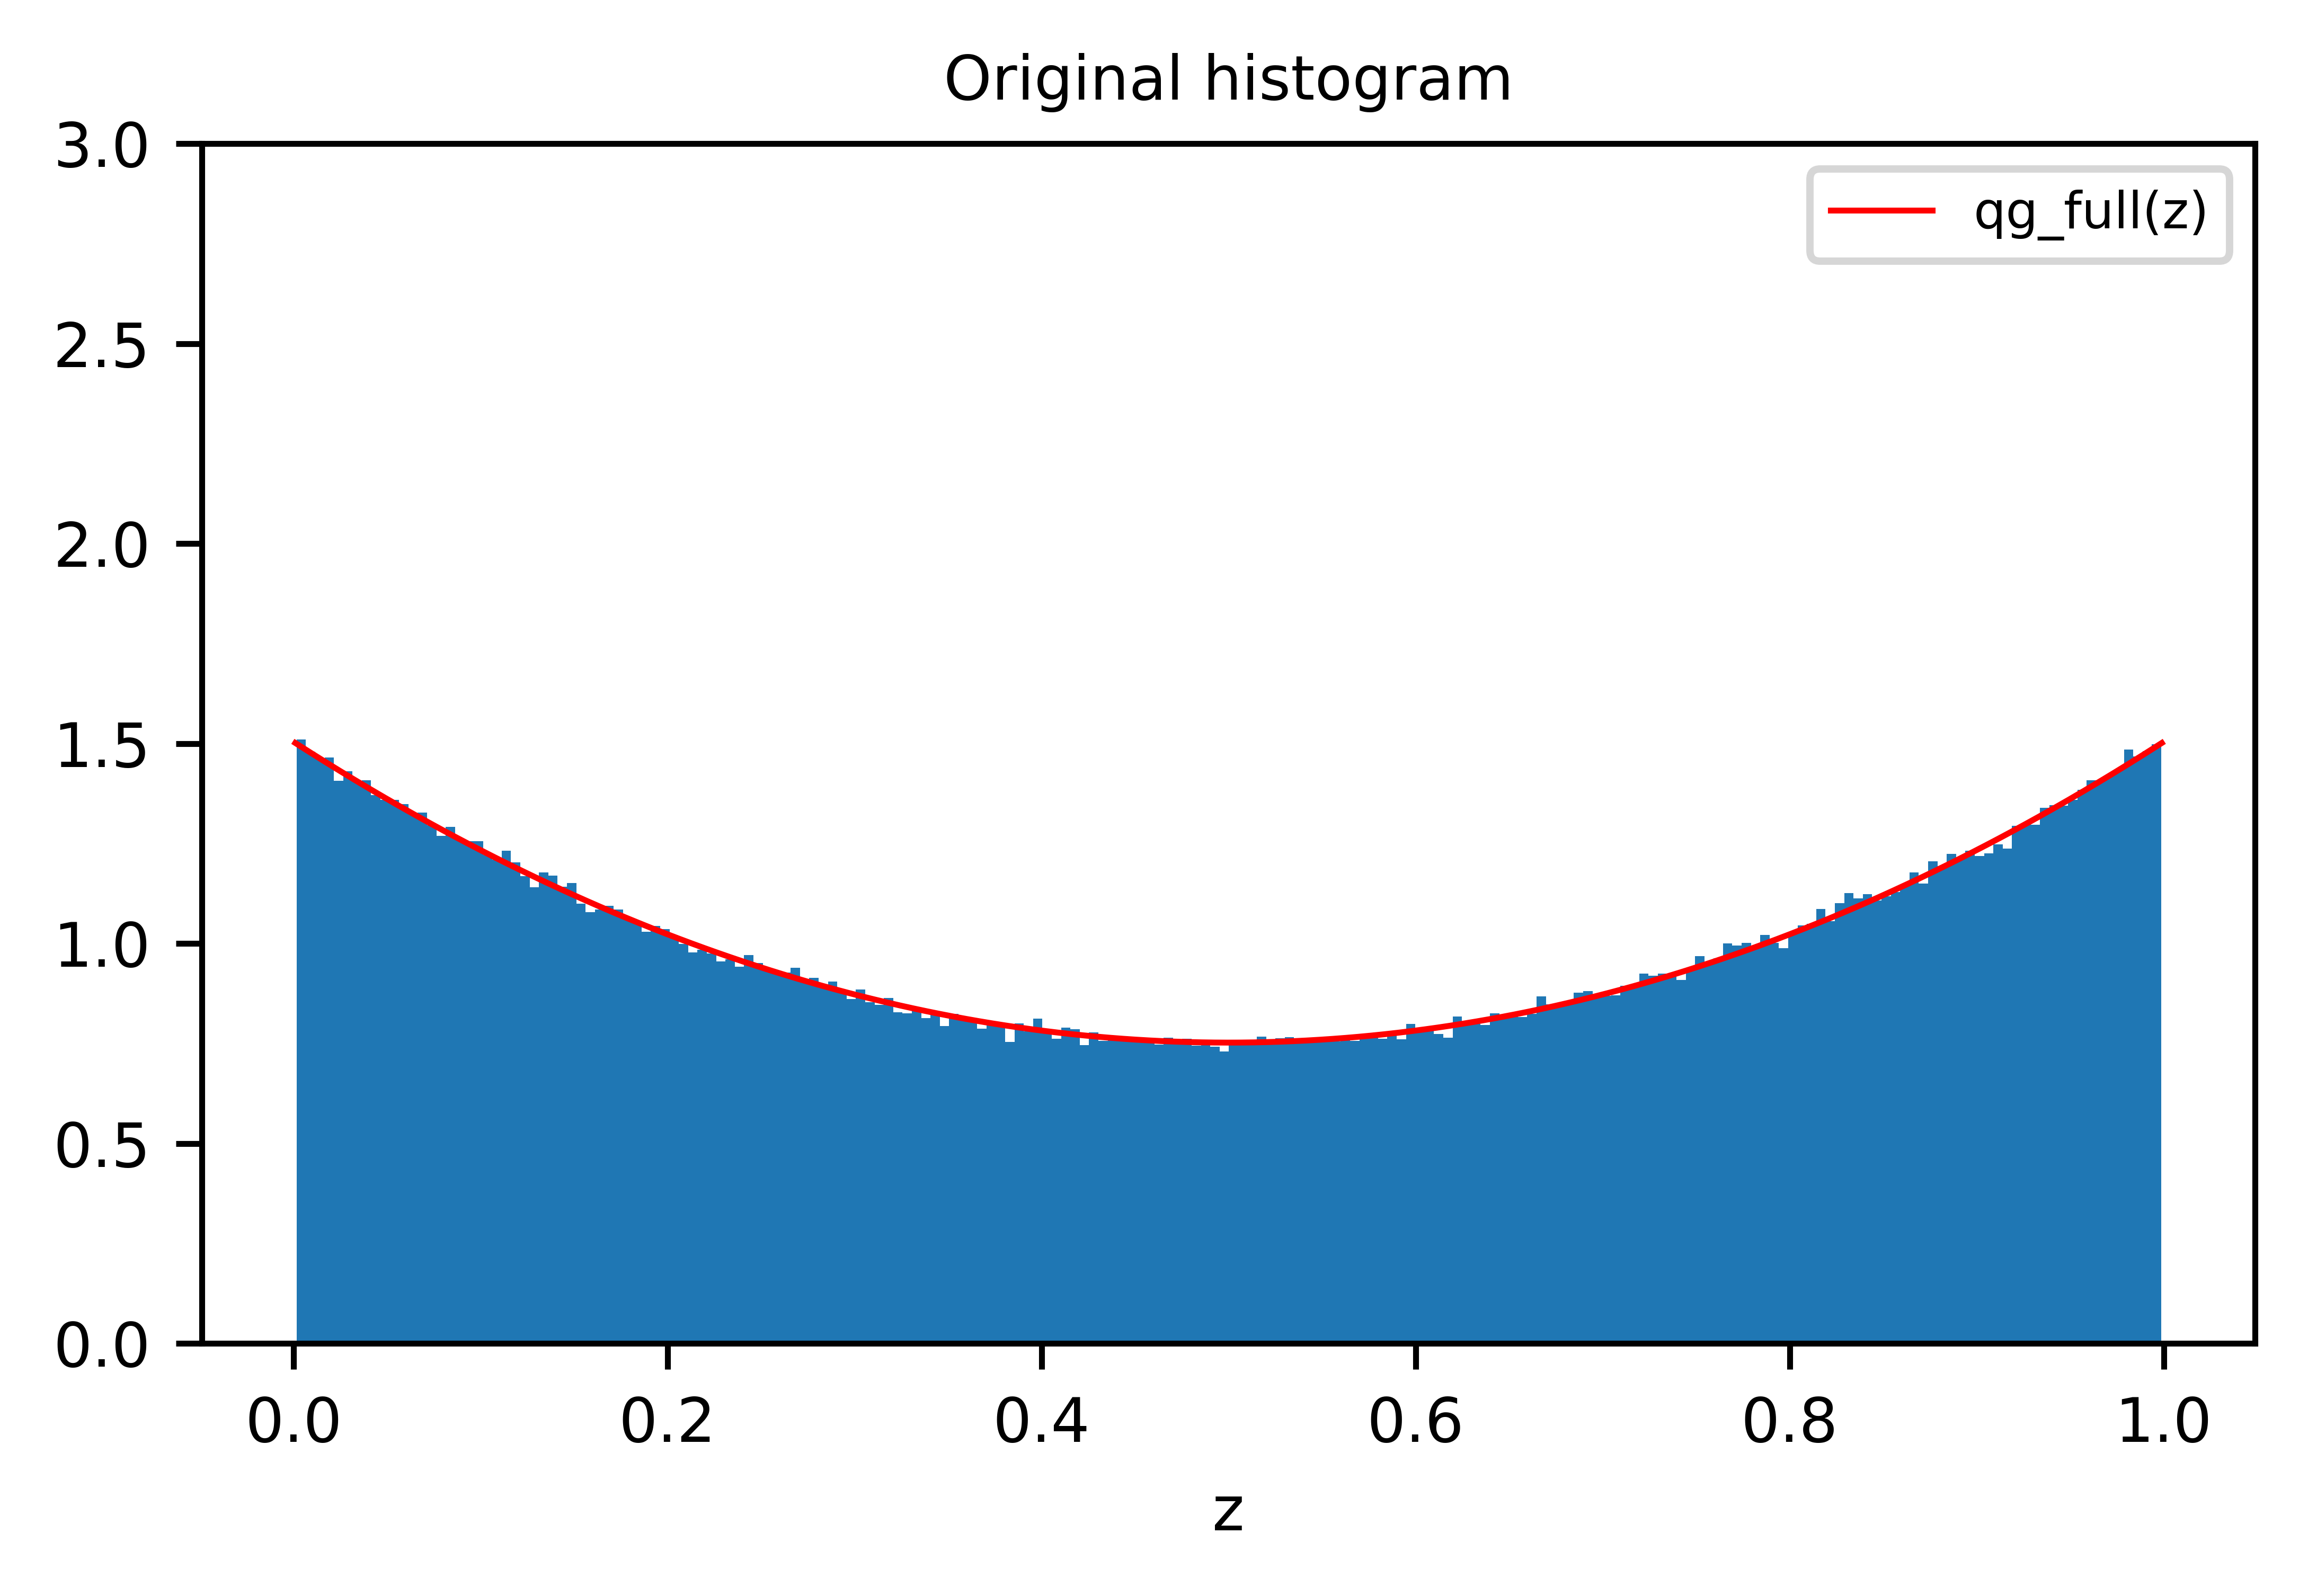
\includegraphics[width=7cm]{pictures/MH_plots/MH_vacuum_qg.png}
    \caption{Probability density of the full \(\hat{P}_{qg}\) splitting function, compared to the histogram of 1,000,000 generated samples.}
    \label{fig: p_qg_splitting}
\end{figure}

\subsubsection{Sampling from the q-qg Vertex in vacuum}
Next up we will solve \autoref{eqn: energyfraction_function_R} for the \qqg splitting function of \autoref{eqn: vacuum_qqg_splitting_function}.
\begin{align}
    \int dz\hat{P}_{qq}(z) &= \int \left(\frac{1+z^2}{1-z} \right)\, dz \nonumber \\
    &= \int \left(\frac{-(z^2+1)}{z-1} \right)\, dz \nonumber \\
    &= \int \left(\frac{-((z-1)(z-1)+2z)}{z-1} \right)\, dz \nonumber \\
    &= \int -(z-1)\, dz - \int \frac{2z}{z-1} \, dz \nonumber \\
    &= \int (1-z) \, dz - \int \frac{2(u+1)}{u} \, du \qquad \text{, where}\; u=z-1 \nonumber \\
    &= \int (1-z) \, dz - \int 2\, dz - \int_a^b \frac{2}{u} \, du \nonumber  \\
    &= -\int (z+1) \, dz - \int \frac{2}{u} \, du \nonumber  \\
    &= -\frac{z^2}{2} - z - 2\left( ln(z-1)\right) 
\end{align}
since this integral has an exact solution, we can solve \autoref{eqn: energyfraction_function_R} for this splitting function,

\begin{align}
    \mathcal{R} \cdot \left[-\frac{z^2}{2} - z - 2\left( ln(z-1)\right) \right]_\epsilon^{1-\epsilon} &= \left[-\frac{z^2}{2} - z - 2\left( ln(z-1)\right) \right]_\epsilon^{y} \nonumber \\
    %\mathcal{R} \cdot \left(-\frac{(1-\epsilon)^2}{2} - (1-\epsilon) - 2 ( ln((1-\epsilon)-1)) \right) &- \mathcal{R} \cdot \left( -\frac{\epsilon^2}{2} - \epsilon - 2 ( ln(\epsilon-1)) \right) \nonumber \\
    %&= \left(-\frac{y^2}{2} - y - 2 ( ln(y-1)) \right) - \left( -\frac{\epsilon^2}{2} - \epsilon - 2 ( ln(\epsilon-1)) \right) \nonumber
    \mathcal{R}\cdot|  \frac{6 \epsilon-3}{2} - 2 ( ln(-\epsilon)) + 2 ( ln(\epsilon-1)) &= -\frac{y^2}{2} - y - 2 ( ln(y-1)) +\frac{\epsilon^2}{2} + \epsilon + 2 ( ln(\epsilon-1)) \nonumber\\
    \frac{y^2}{2} + y + ln \left( \frac{y-1}{\epsilon-1}\right)^2  &= -\left(\mathcal{R} \cdot \frac{6 \epsilon-3}{2} + \frac{-\epsilon^2-4 \epsilon}{2}\right) - ln\left(\frac{1-\epsilon}{\epsilon}\right)^{2\mathcal{R}}
\end{align}
This equation is difficult to solve, so we will try Metropolis-Hastings algorithm for approximating the results.
The \qqg splitting function is \(\hat{P}_{qq}(z) = \frac{1+z^2}{1-z}\), we will try a dummy function \(\hat{P}_{qq \text{dummy}} = \frac{-2}{z-1}\).
The integral is simply,
\begin{align}
    \int(\frac{-2}{z-1})dz = -2 ln(z-1)
\end{align}
Now we will try to solve \autoref{eqn: energyfraction_function_R}, with this dummy splitting function, 
\begin{align}
    \mathcal{R}\cdot \left[-2 ln(z-1)\right]_{\epsilon}^{1-\epsilon} &= \left[-2 ln(z-1)\right]_{\epsilon}^{y} \nonumber \\
    \mathcal{R}\cdot \left(-2 ln((1-\epsilon)-1) + 2 ln(\epsilon-1) \right) &= \left(-2 ln(y-1) + 2 ln(\epsilon-1) \right) \nonumber \\
    \mathcal{R}\cdot ln\left(\frac{1-\epsilon}{\epsilon} \right) &= - ln(y-1) + ln(\epsilon-1)
\end{align}
moving terms and exponentiating, 
\begin{align}
    ln(y-1) &= ln(\epsilon-1) - ln\left(\frac{1-\epsilon}{\epsilon} \right)^{\mathcal{R}} \nonumber \\
    y-1 &= \frac{e^{ln(\epsilon-1)}}{e^{ln(\frac{1-\epsilon}{\epsilon})^{\mathcal{R}}}} \nonumber \\
    y &= \frac{(\epsilon-1)}{(\frac{1-\epsilon}{\epsilon})^{\mathcal{R}}} +1
\end{align}
Following the same procedure as in Section \ref{sec: metropolis_hastings}, we can generate our MH corrected histogram, for the \(\hat{P}_{qq}\) splitting function. The plot is given in \autoref{fig: MH_corrected_p_qq_splitting}.
\begin{figure}[ht]
    \centering
    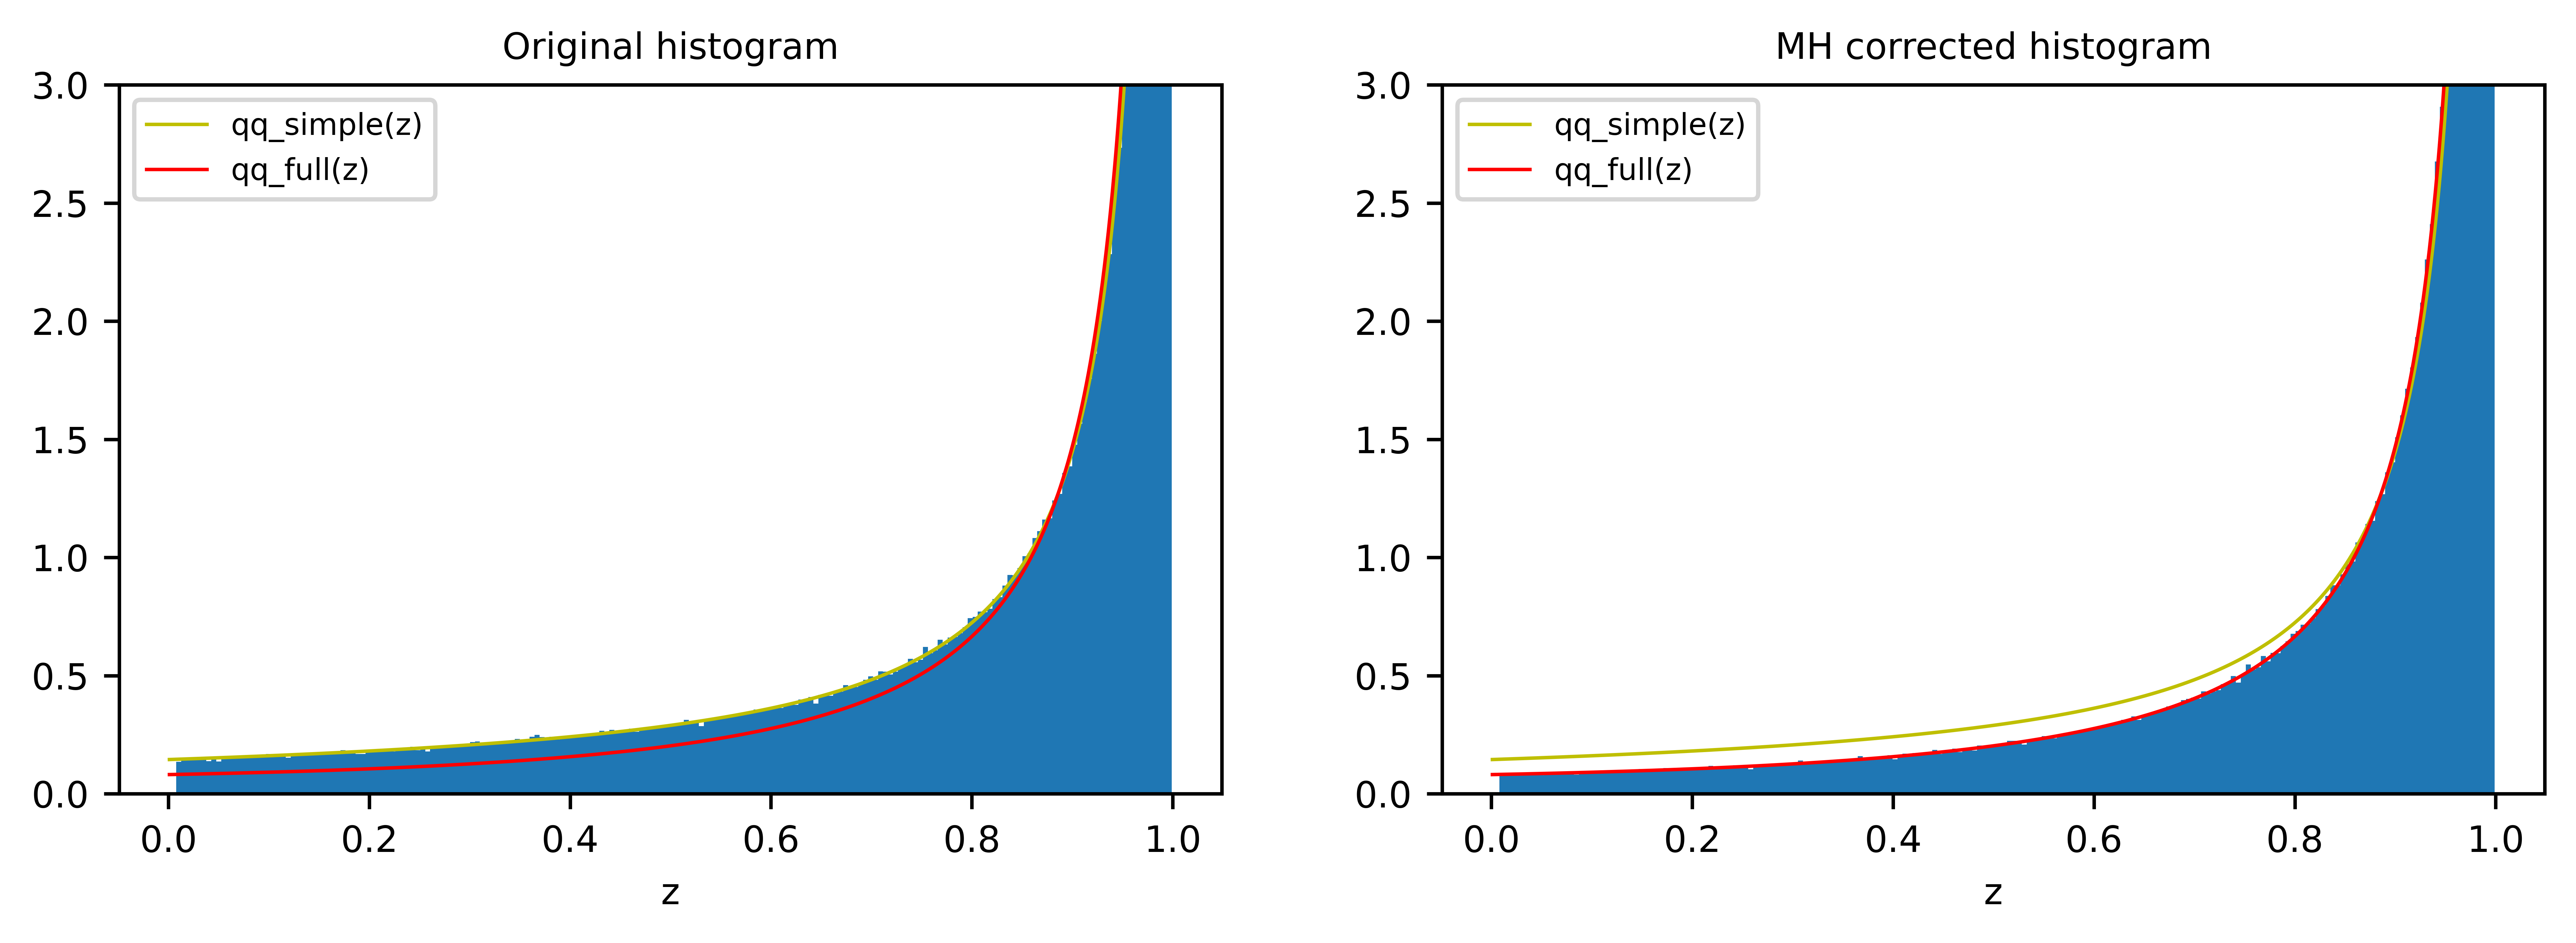
\includegraphics[width=14cm]{pictures/MH_plots/MH_vacuum_qq.png}
    \caption{Probability density of the full \(\hat{P}_{qq}\) splitting function, compared to the density histogram of the dummy splitting function, and the Metropolis-Hastings corrected results. Simulated with \(1,000,000\) points, and an acceptance rate of \(0.89\).}
    \label{fig: MH_corrected_p_qq_splitting}
\end{figure}

\subsection{Monte Carlo implementation}
The  code for running the Monte Carlo is given in \textcolor{red}{reference appendix where code is}, but a brief overview of the logical structure of the main \textit{generate\_shower} subprogram will be given here. The reason is that this is where all of the actual physics is applied, while the rest of the program is for plotting, defining variables, and creating the \textit{parton-objects} and \textit{shower-objects}. 

For each individual shower, the program initiates \textit{generate\_shower} which is outlined here:
\begin{enumerate}[Step 1:]
    \item The program start by creating the initial object of the \textit{parton-class}, and a single objects of the \textit{shower-class}. The former will be used directly in the splitting process, while the latter is simply used to store information about the particular shower.
    \item If \textit{t\_max} is not passed to the function, then it must be calculated now.
    \item After this a \textit{while True} loop is initiated, which is terminated when the shower terminates.
    \begin{enumerate}[{while} i)]
    \item The loop starts by calculating the expected splitting intervals by calling the \textit{advance\_time} function, which calculates \textit{delta\_t\_quark} and \textit{delta\_t\_gluon}, from \autoref{eqn: sudakov_splitting_interval_quarks} and \autoref{eqn: sudakov_splitting_interval_gluons}, respectively.
    \item It is now necessary to determine if the evolution interval is large enough to allow the different splittings. This is done in a \textit{if, elif, else} statement,
    \begin{itemize}
        \item \textit{if ((t+delta\_t\_quark) < t\_max) and ((t+delta\_t\_gluon) < t\_max):}\newline
        When this condition is met, the evolution interval is large enough for both quark and gluon splittings to occur. The \textit{select\_splitting} subprogram is therefore called to determine which type of parton to split, based on \autoref{eqn: parton_selection_ratios} and the available partons. The interval is then evolved accordingly,a and a suitable parton is randomly drafted. If there are no suitable partons, the loop is terminated.
        \item \textit{elif ((t+delta\_t\_quark) >= t\_max) and ((t+delta\_t\_gluon) < t\_max):} \newline
        When this condition is met, the interval is only large enough to split a gluon. A gluon is then randomly selected, and the interval is evolved accordingly. If no available gluons, the loop is terminated.
        \item \textit{else:} \newline
        If this condition is reached, then \(t>t_{max}\) and the shower is terminated by breaking out of the while loop.
    \end{itemize}
    \item The program has now chosen parton to split, and we need to remove it from the list of final partons, and split it. If the splitting parton is a gluon, we first need to determine how to split it, as given in \autoref{eqn: gluon_splitting_selection_ratios}. When the splitting procedure is determined, the energy fractions of the new partons are calculated by the methods outlined in \autoref{sec: metropolis_hastings}.
    \item Finally the two new partons are created according to the selections done in the splitting process. If the momentum fractions of the new partons are high enough, they are appended to the splitting list. The loop then starts again from the top.
    \end{enumerate}
\item The shower has now terminated, and we write the various properties of the shower to the \textit{shower-object}, before ending the \textit{generate\_shower} program.
\end{enumerate}

\subsection{Validating MC Results for vacuum shower}
\subsubsection{Comparison with Dasgupta results}
Now the time has come to validate the results of our shower program. An initial check of the validity of the program can be done by comparing with the results from figure 2 of \cite{Dasgupta_2015}, in which the inclusive distribution has been plotted for fixed values of the evolution variable, \( t = 0.04, 0.1, 0.2, 0.3\).
\begin{figure}[ht]
    \centering
    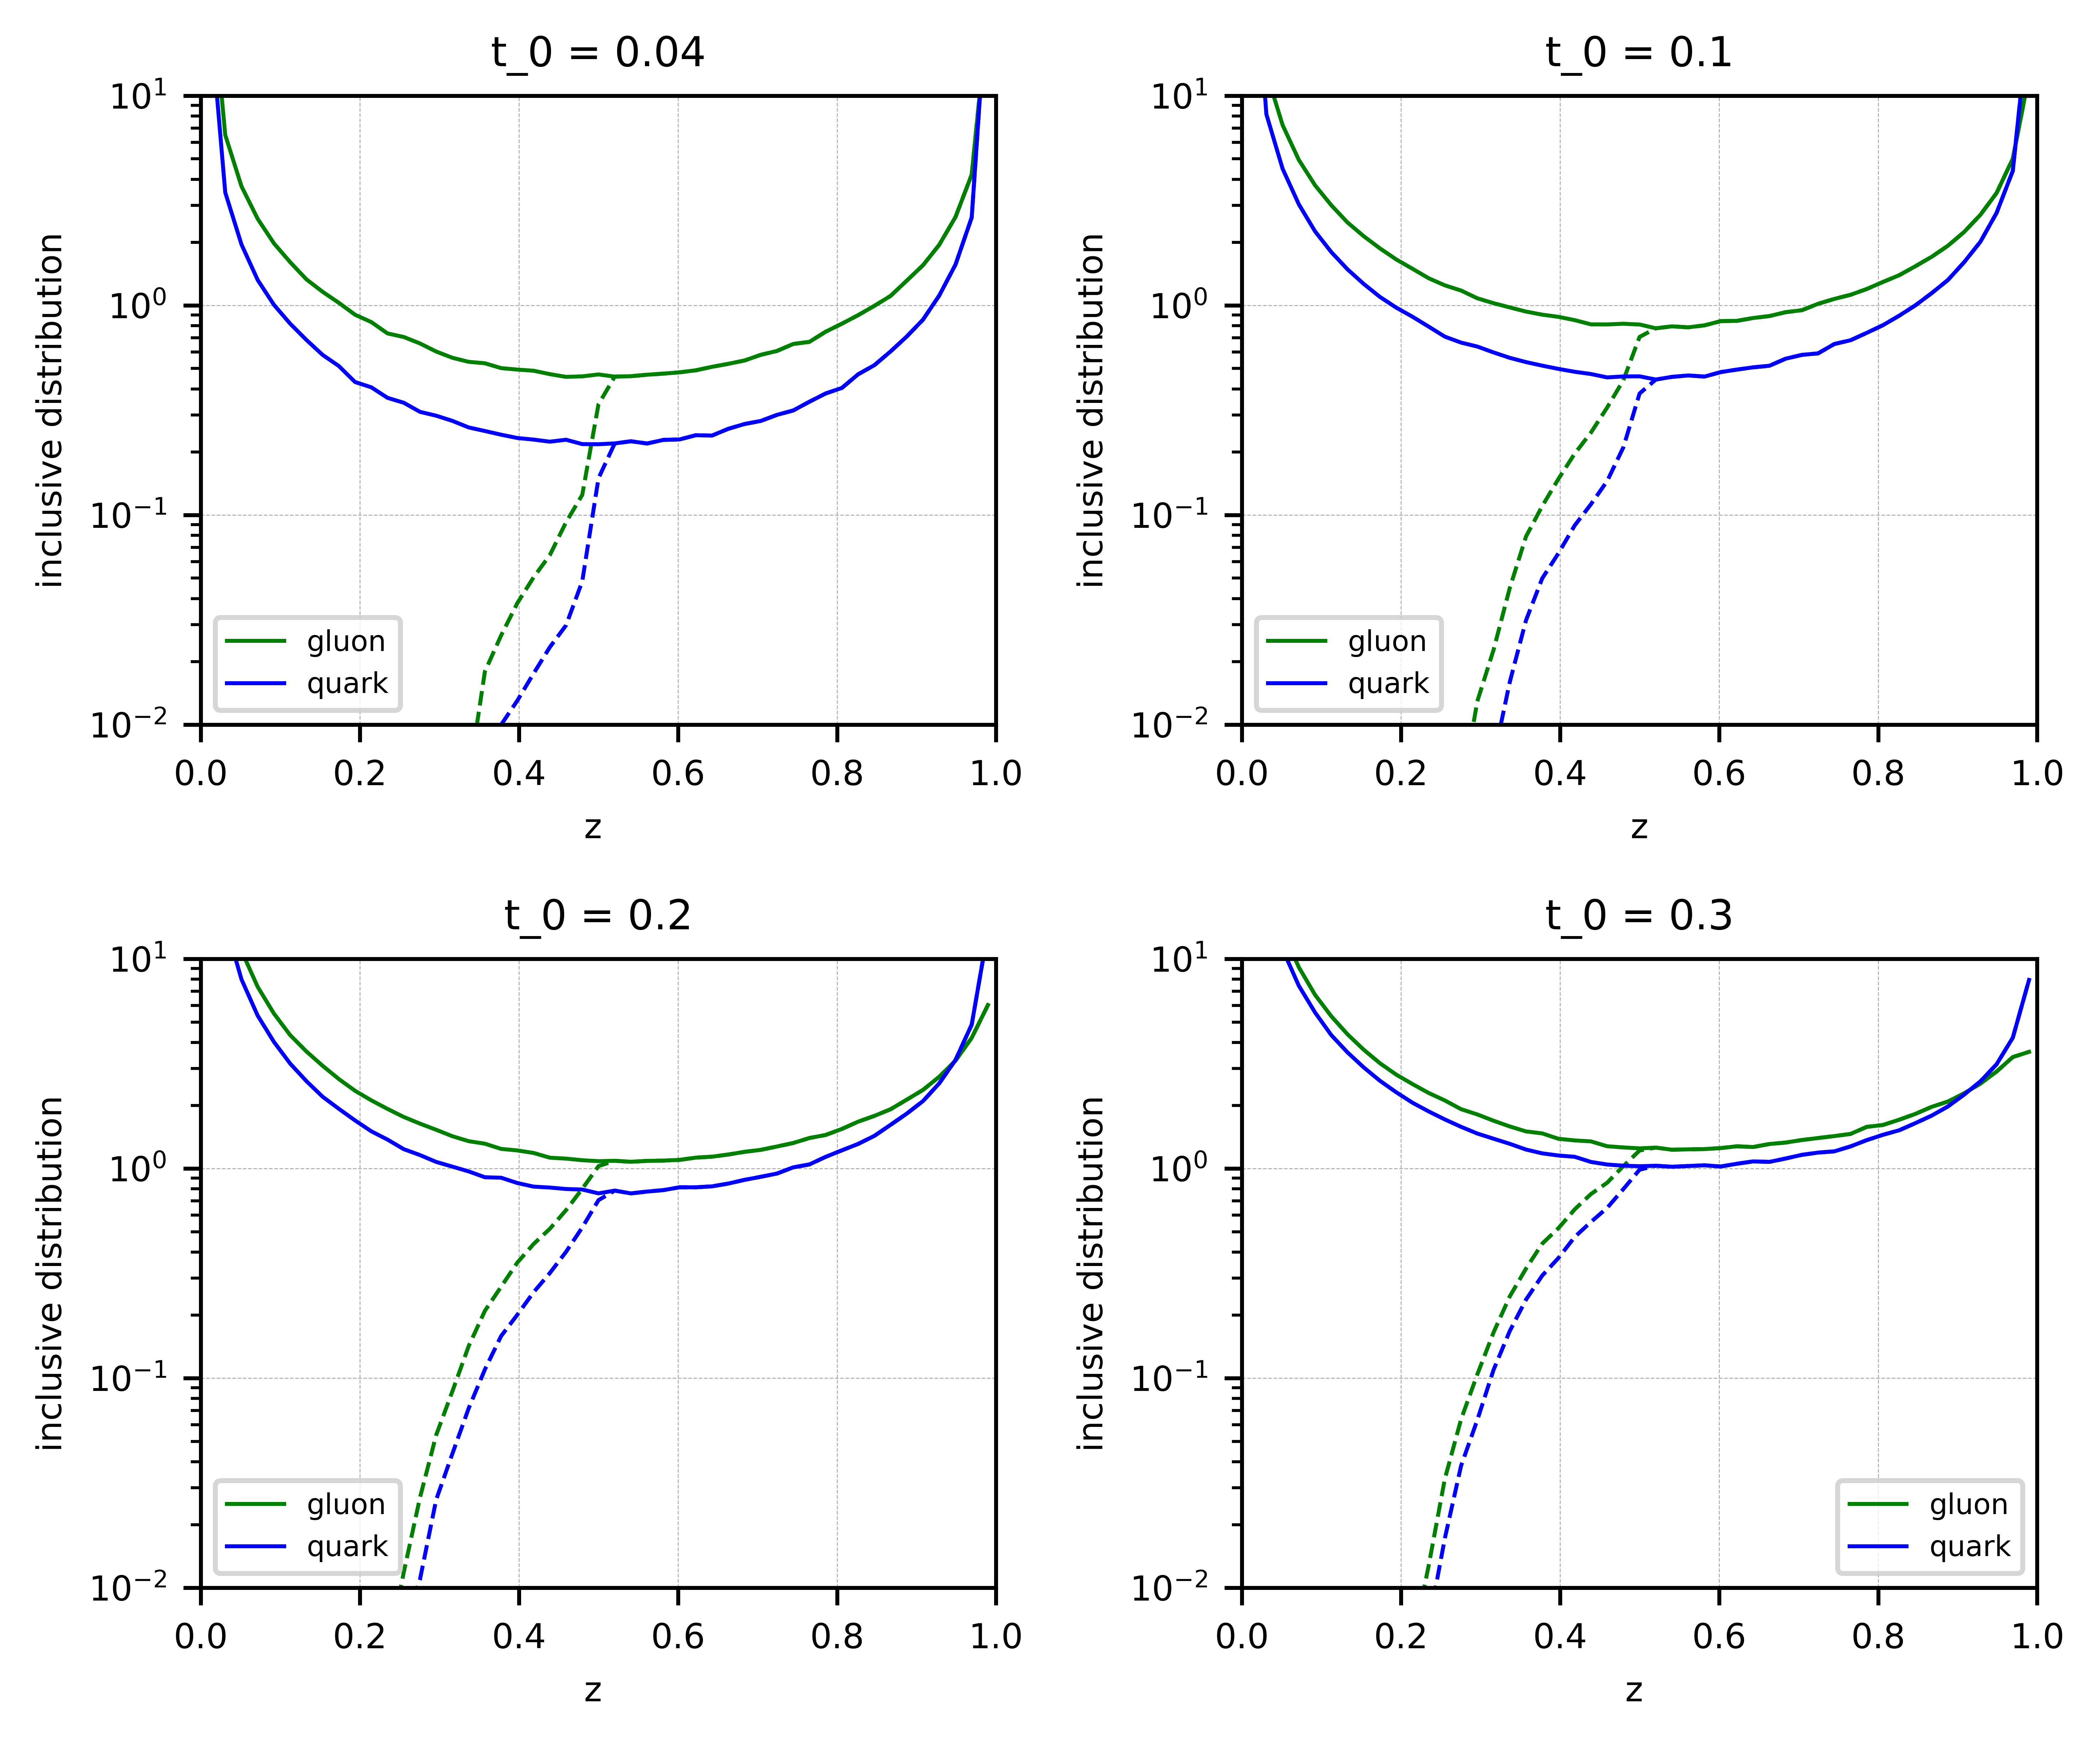
\includegraphics[width=12cm]{pictures/distributions/vacuum_quarkgluon_dasgupta_500k_minz_incldist.png}
    \caption{Inclusive spectrum generated from the Monte Carlo program with quarks and gluons in vacuum. Simulated with \(500,000\) showers for both initial quark and initial gluon. }
    \label{fig: vacuum_distribution_quark_and_gluon}
\end{figure}

\subsubsection{Comparison with analytical results}
\textcolor{red}{Reference my own analytical solution from sec 1.}
From Appendix B of \cite{Energy_flow_medium_cascade_2016} we are presented with an analytical solution to the DGLAP cascade in equation B7, 
\begin{equation}\label{DGLAP_solution_energyflowmedium}
    D(x,t) = \frac{1}{2} \left( \frac{t}{\pi \ln^3\frac{1}{x}}\right)^{1/4} \, \exp \left(-\gamma t +2 \sqrt{t \ln\frac{1}{x}}\right) 
\end{equation}
Plotting this solution alongside the pure gluon shower in vacuum, we can compare the results as follows, 
\begin{figure}[ht]
    \centering
    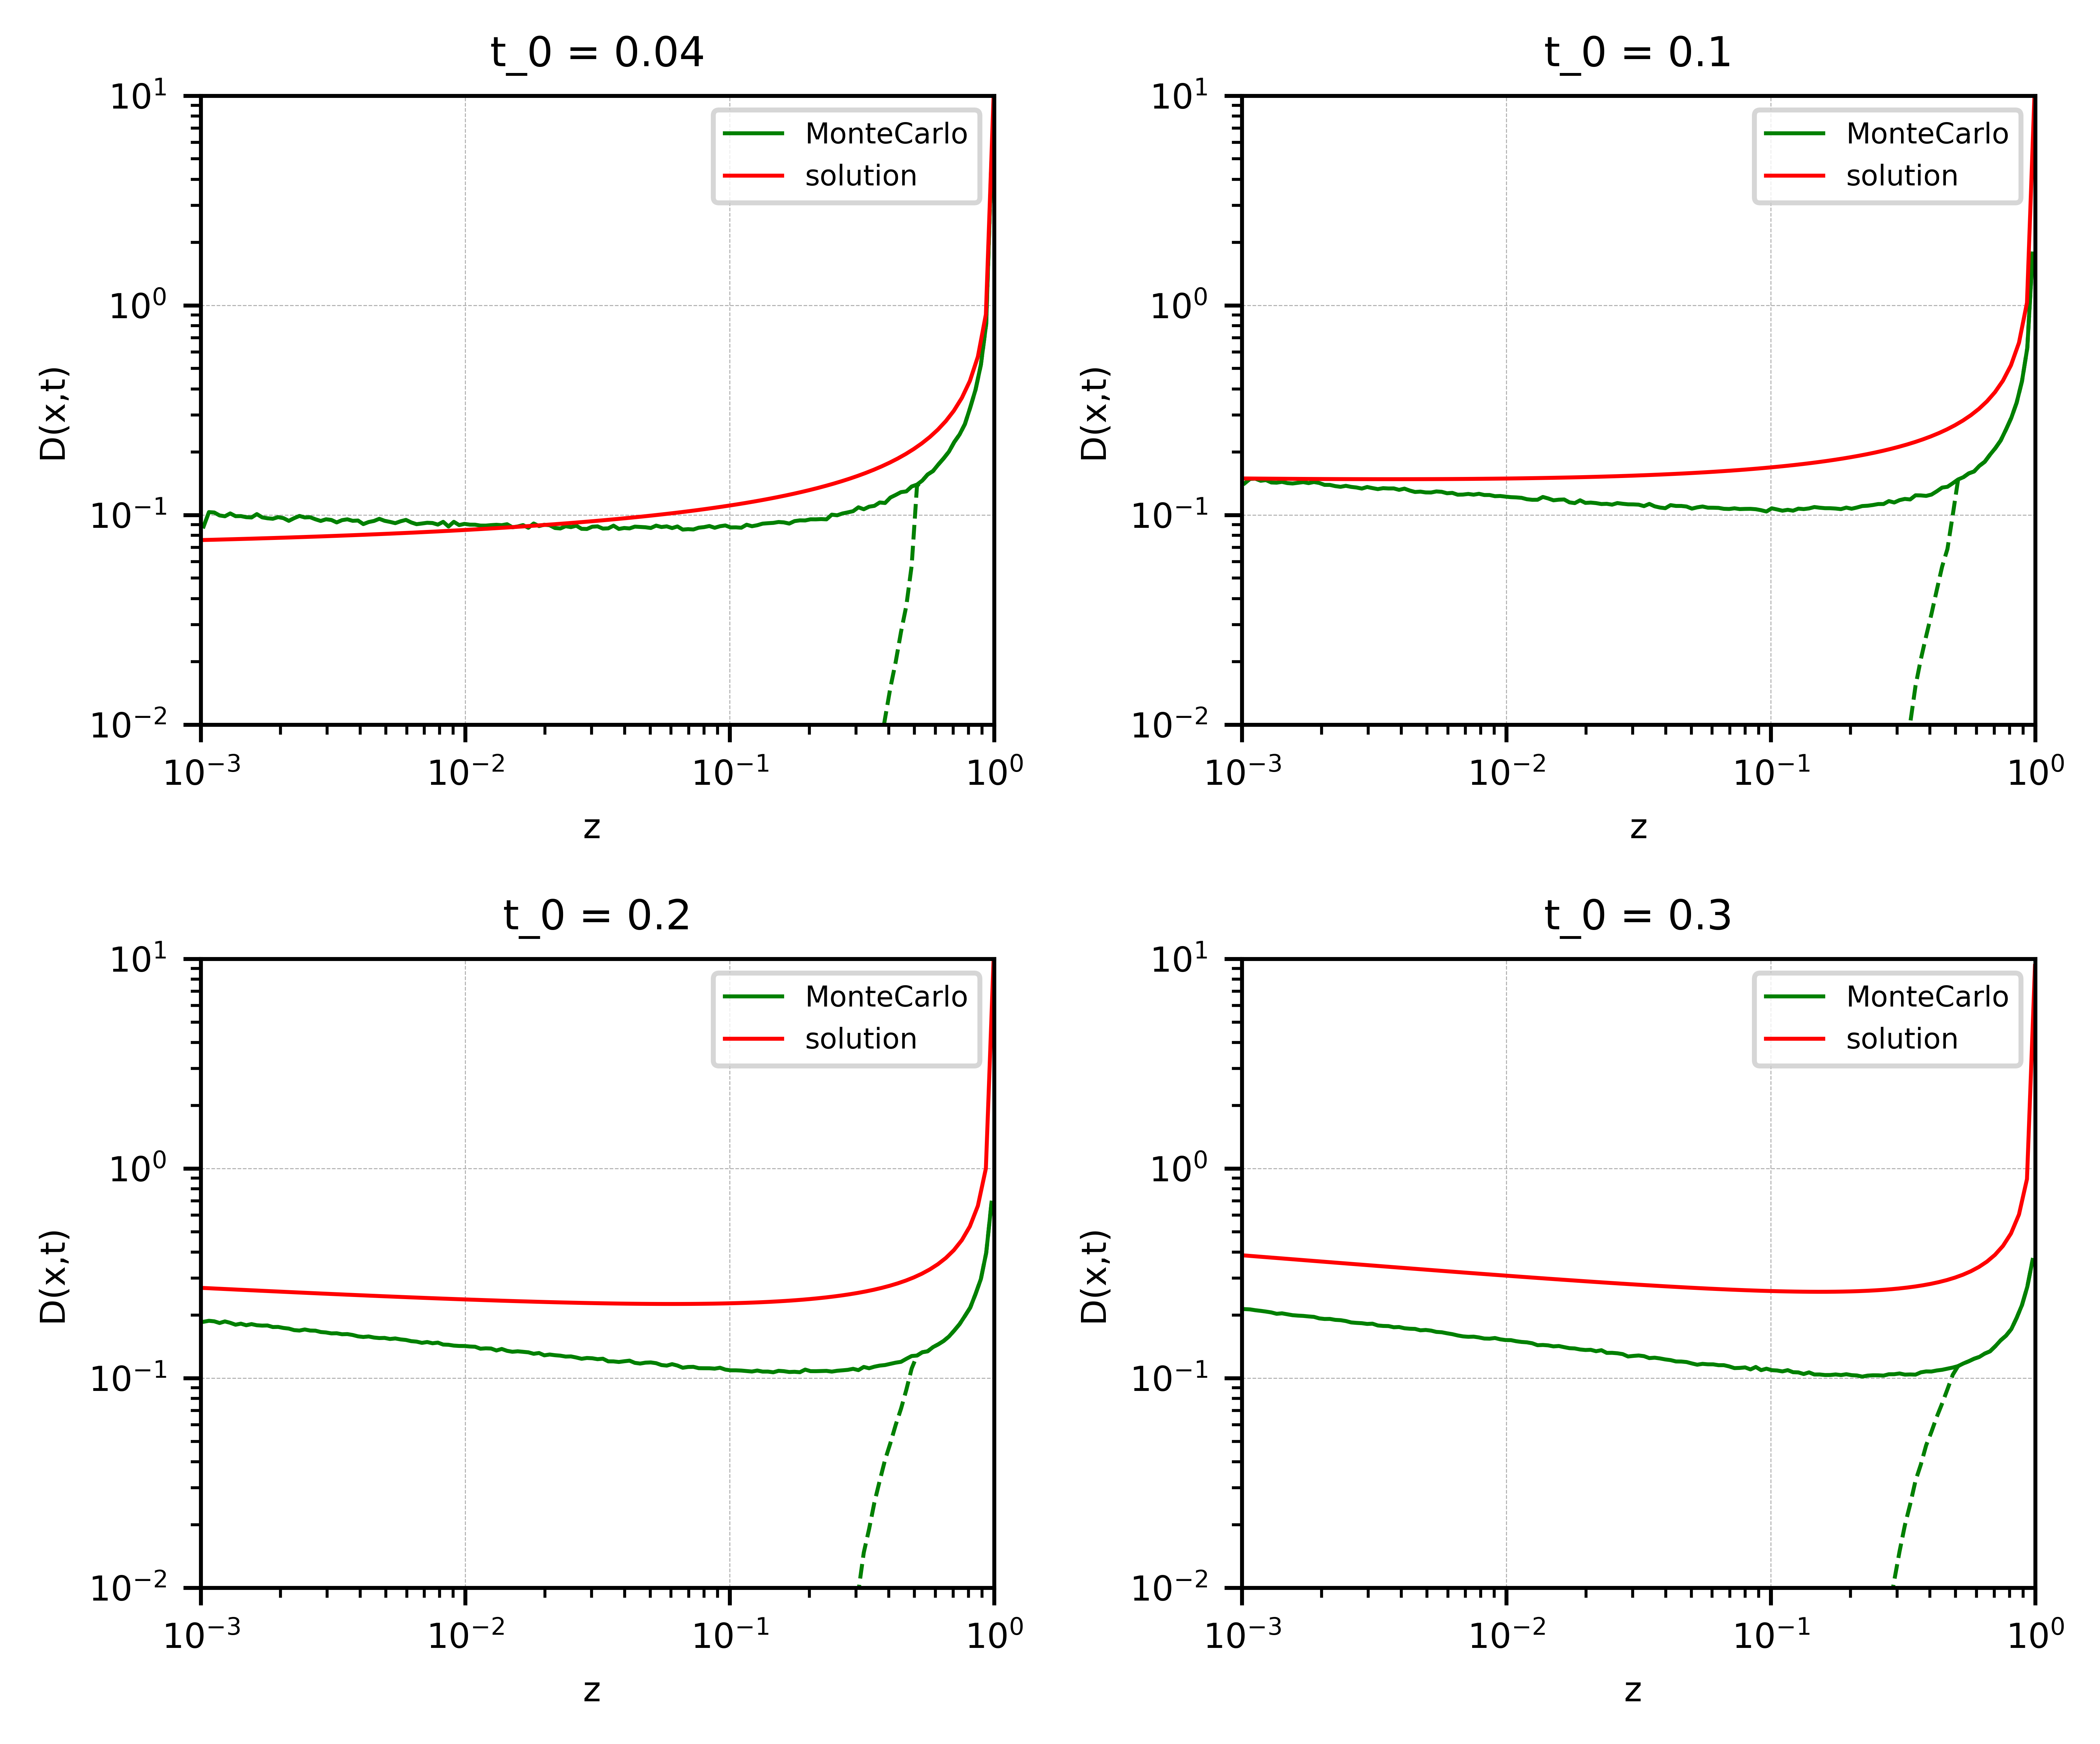
\includegraphics[width=12cm]{pictures/distributions/vacuum_shower_simple_ggg_500k_minz0_MCandAnalytical.png}
    \caption{Inclusive spectrum generated from the Monte Carlo vacuum program plotted with the analytical solution. MC simulated with \(500,000\) showers using the simplified \(P_{ggg}\) splitting function, and no quarks.}
    \label{fig: vacuum_MCandAnalytical_comparison}
\end{figure}

\newpage
\section{Parton showers in medium}
We will now go on to gluon splittings in a medium. 

\subsection{Evolution interval}
As discussed in \autoref{sec: BDMPS_theory}, the medium cascade evolves according to the actual time, up to the characteristic time which is the time it takes for the initial parton to radiate most of its energy into soft gluons. The boundaries of the medium evolution can therefore be noted as, 
\begin{align}\label{eqn: medium_evolution_boundaries}
    0 < t < t_* = \frac{\pi}{\alpha_S N_C} \sqrt{\frac{E}{\hat q}} \nonumber \\
    0 < \frac{t}{t_*} = \tau < 1
\end{align}
Determining the probable splitting time can again be done from the Sudakov form-factor which was introduced in \autoref{eqn: BDMPS_sudakov} for the medium evolution in \autoref{sec: medium_sudakov}, and we can therefore follow the procedure of \autoref{sec: determining_evolution_time_from_sudakov} to determine a probable branching interval \(\Delta t = t-t_0\). Doing this in terms of \(\tau\), such that \(\Delta \tau = \frac{\Delta t}{t_*}\), and  \(\frac{\Delta t}{t_*(x)} = \frac{\Delta t}{t_* \, \sqrt{x}} = \frac{\Delta \tau}{\sqrt{x}}\). The evolution probability takes the form,
\begin{align}
    \mathcal{P}(\Delta t) &= \frac{\Delta(t_0)}{\Delta(t)} = \exp \left(- \frac{\Delta t}{t_*(x)} \int_\epsilon^{1-\epsilon} \, dz\, z \mathcal{K}(z) \right) \nonumber \\
    \mathcal{P}(\Delta \tau) &= \frac{\Delta(\tau_0)}{\Delta(\tau)} = \exp \left(- \frac{\Delta \tau}{\sqrt{x}} \int_\epsilon^{1-\epsilon} \, dz\, z \mathcal{K}(z) \right)
\end{align}
Exchanging the probability with a randomly generated number \(\mathcal{R}\in (0,1)\), we obtain
\begin{align}
    \Delta \tau &= -\frac{\sqrt{x}\,\ln(\mathcal{R}) }{\int_\epsilon^{1-\epsilon} \, dz\, z \mathcal{K}(z)} \nonumber \\
    &= -\frac{\sqrt{x}\,\ln(\mathcal{R}) }{\int_\epsilon^{1-\epsilon} \, dz\, z \mathcal{K}(z)} 
\end{align}
from the symmetry of the splitting kernel, we have \(\int_0^1 \, dz\, z \mathcal{K}(z) = \frac{1}{2} \int_0^1 \, dz \mathcal{K}(z)\), and the probably evolution interval can be therefore be determined from \autoref{eqn: BDMPS_probable_branching_interval_tau}.
\begin{equation}\label{eqn: BDMPS_probable_branching_interval_tau}
    \Delta \tau = -\frac{2\, \sqrt{x}\cdot \ln(\mathcal{R}) }{\int_\epsilon^{1-\epsilon} \, dz \mathcal{K}(z)} 
\end{equation}

\subsection{Medium splitting functions}
Energy fractions are determined in the same manner as for the vacuum cascades, and we can therefore reuse \autoref{eqn: energyfraction_function_R}. 
\textcolor{red}{Do own derivation?}
The full medium splitting kernels are given by equation 2.9-2.12 of Universal QG Cascade  \cite{Universal_quark_gluon_ratio_in_medium-induced_parton_cascade}, as 
\begin{align}
    \mathcal{K}_{gg}(z) &= \frac{1}{2} \, 2\, C_A \, \frac{(1-z(1-z))^2}{z(1-z)} \, \sqrt{\frac{(1-z)C_A + z^2 \, C_A}{z(1-z)}}  \label{eqn: medium_ggg_splittingfunction} \\
    \mathcal{K}_{qg}(z) &= \frac{1}{2} \, 2\, N_f T_F \left(z^2 + (1-z)^2 \right) \, \sqrt{\frac{C_F - z(1-z) \, C_A}{z(1-z)}} \label{eqn: medium_qgg_splittingfunction} \\
    \mathcal{K}_{qq}(z) &= \frac{1}{2} \, C_F \, \frac{1+z^2}{1-z} \, \sqrt{\frac{z\, C_A + (1-z)^2 \, C_F}{z(1-z)}} \label{eqn: medium_qqg_splittingfunction}
\end{align}

\subsubsection{ggg medium splitting function}
For gluons in medium, it will be sufficient to work with the simplified splitting kernel as presented in \autoref{eqn: ggg_medium_reduced_kernel}. The reasoning is simply that \label{eqn: BDMPS_solution_startingpoint} which was the starting point for our analytical solution, is only dependent on the simplified splitting kernel.
It is also worth noting that all factors \(C_A\) are already absorbed into \(\tau\).

The problem of sampling values directly from the splitting function is still present, so returning to \autoref{eqn: probability_density_for_splitting}, we again need to solve \autoref{eqn: energyfraction_function_R}. 
\begin{equation}\tag{\ref{eqn: energyfraction_function_R}}
    \mathcal{R} \cdot \int_\epsilon^{1-\epsilon} dz \, \mathcal{K}(z) = \int_\epsilon^{y}dz \, \mathcal{K}(z)
\end{equation}
The integral can be generally shown to be, 
\begin{align}
    \int_a^b \frac{1}{(z(1-z))^{3/2}}dz &= \left[ \frac{4z-2}{\sqrt{-z(z-1)}} \right]_a^b
\end{align}
which means that we can evaluate \autoref{eqn: energyfraction_function_R} as,
\begin{align}
    \mathcal{R} \int_\epsilon^{1-\epsilon} dz \, \frac{1}{(z(1-z))^{3/2}} &= \int_\epsilon^{y} \frac{1}{(z(1-z))^{3/2}} \nonumber \\
    \mathcal{R} \left(  \frac{4(1-\epsilon)-2}{\sqrt{-(1-\epsilon)((1-\epsilon)-1)}} - \frac{4\epsilon-2}{\sqrt{-\epsilon(\epsilon-1)}} \right) &= \frac{4y-2}{\sqrt{-y(y-1)}} - \frac{4\epsilon-2}{\sqrt{-\epsilon(\epsilon-1)}} \nonumber\\
    \mathcal{R} \left(  \frac{2-4\epsilon}{\sqrt{\epsilon(1-\epsilon)}} - \frac{4\epsilon-2}{\sqrt{\epsilon(1-\epsilon)}} \right) &= \frac{4y-2}{\sqrt{-y(y-1)}} - \frac{4\epsilon-2}{\sqrt{-\epsilon(\epsilon-1)}} \nonumber\\
    \mathcal{R} \left(  \frac{4-8\epsilon}{\sqrt{\epsilon(1-\epsilon)}} \right) - \frac{2-4\epsilon}{\sqrt{\epsilon(1-\epsilon)}} &= \frac{4y-2}{\sqrt{-y(y-1)}} 
\end{align}
The term on the l.h.s can be written in terms of the integral again and assigned to a variable \(a\), 
\begin{equation}
    a = \int_\epsilon^{1-\epsilon} dz \cdot \left(\mathcal{R} - \frac{1}{2} \right) = \mathcal{R} \left(  \frac{4-8\epsilon}{\sqrt{\epsilon(1-\epsilon)}} \right) + \frac{2-4\epsilon}{\sqrt{\epsilon(1-\epsilon)}}
\end{equation}
Inserting this \(a\), the remainder of the equation can be solved using Mathematica,
\begin{align}\label{eqn: medium_gg_sampling}
    y &= \frac{16 + a^2 \mp a \sqrt{16 + a^2}}{2 (16 + a^2)} \nonumber\\
    y &= \frac{1}{2} \mp \frac{a \sqrt{16 + a^2}}{2 (16 + a^2)} \nonumber\\
    y &= \frac{1}{2} \mp \frac{a }{2 \sqrt{16 + a^2}}
\end{align}
And we now have a method for randomly sampling from the simplified splitting kernel. 
\begin{figure}[ht]
    \centering
    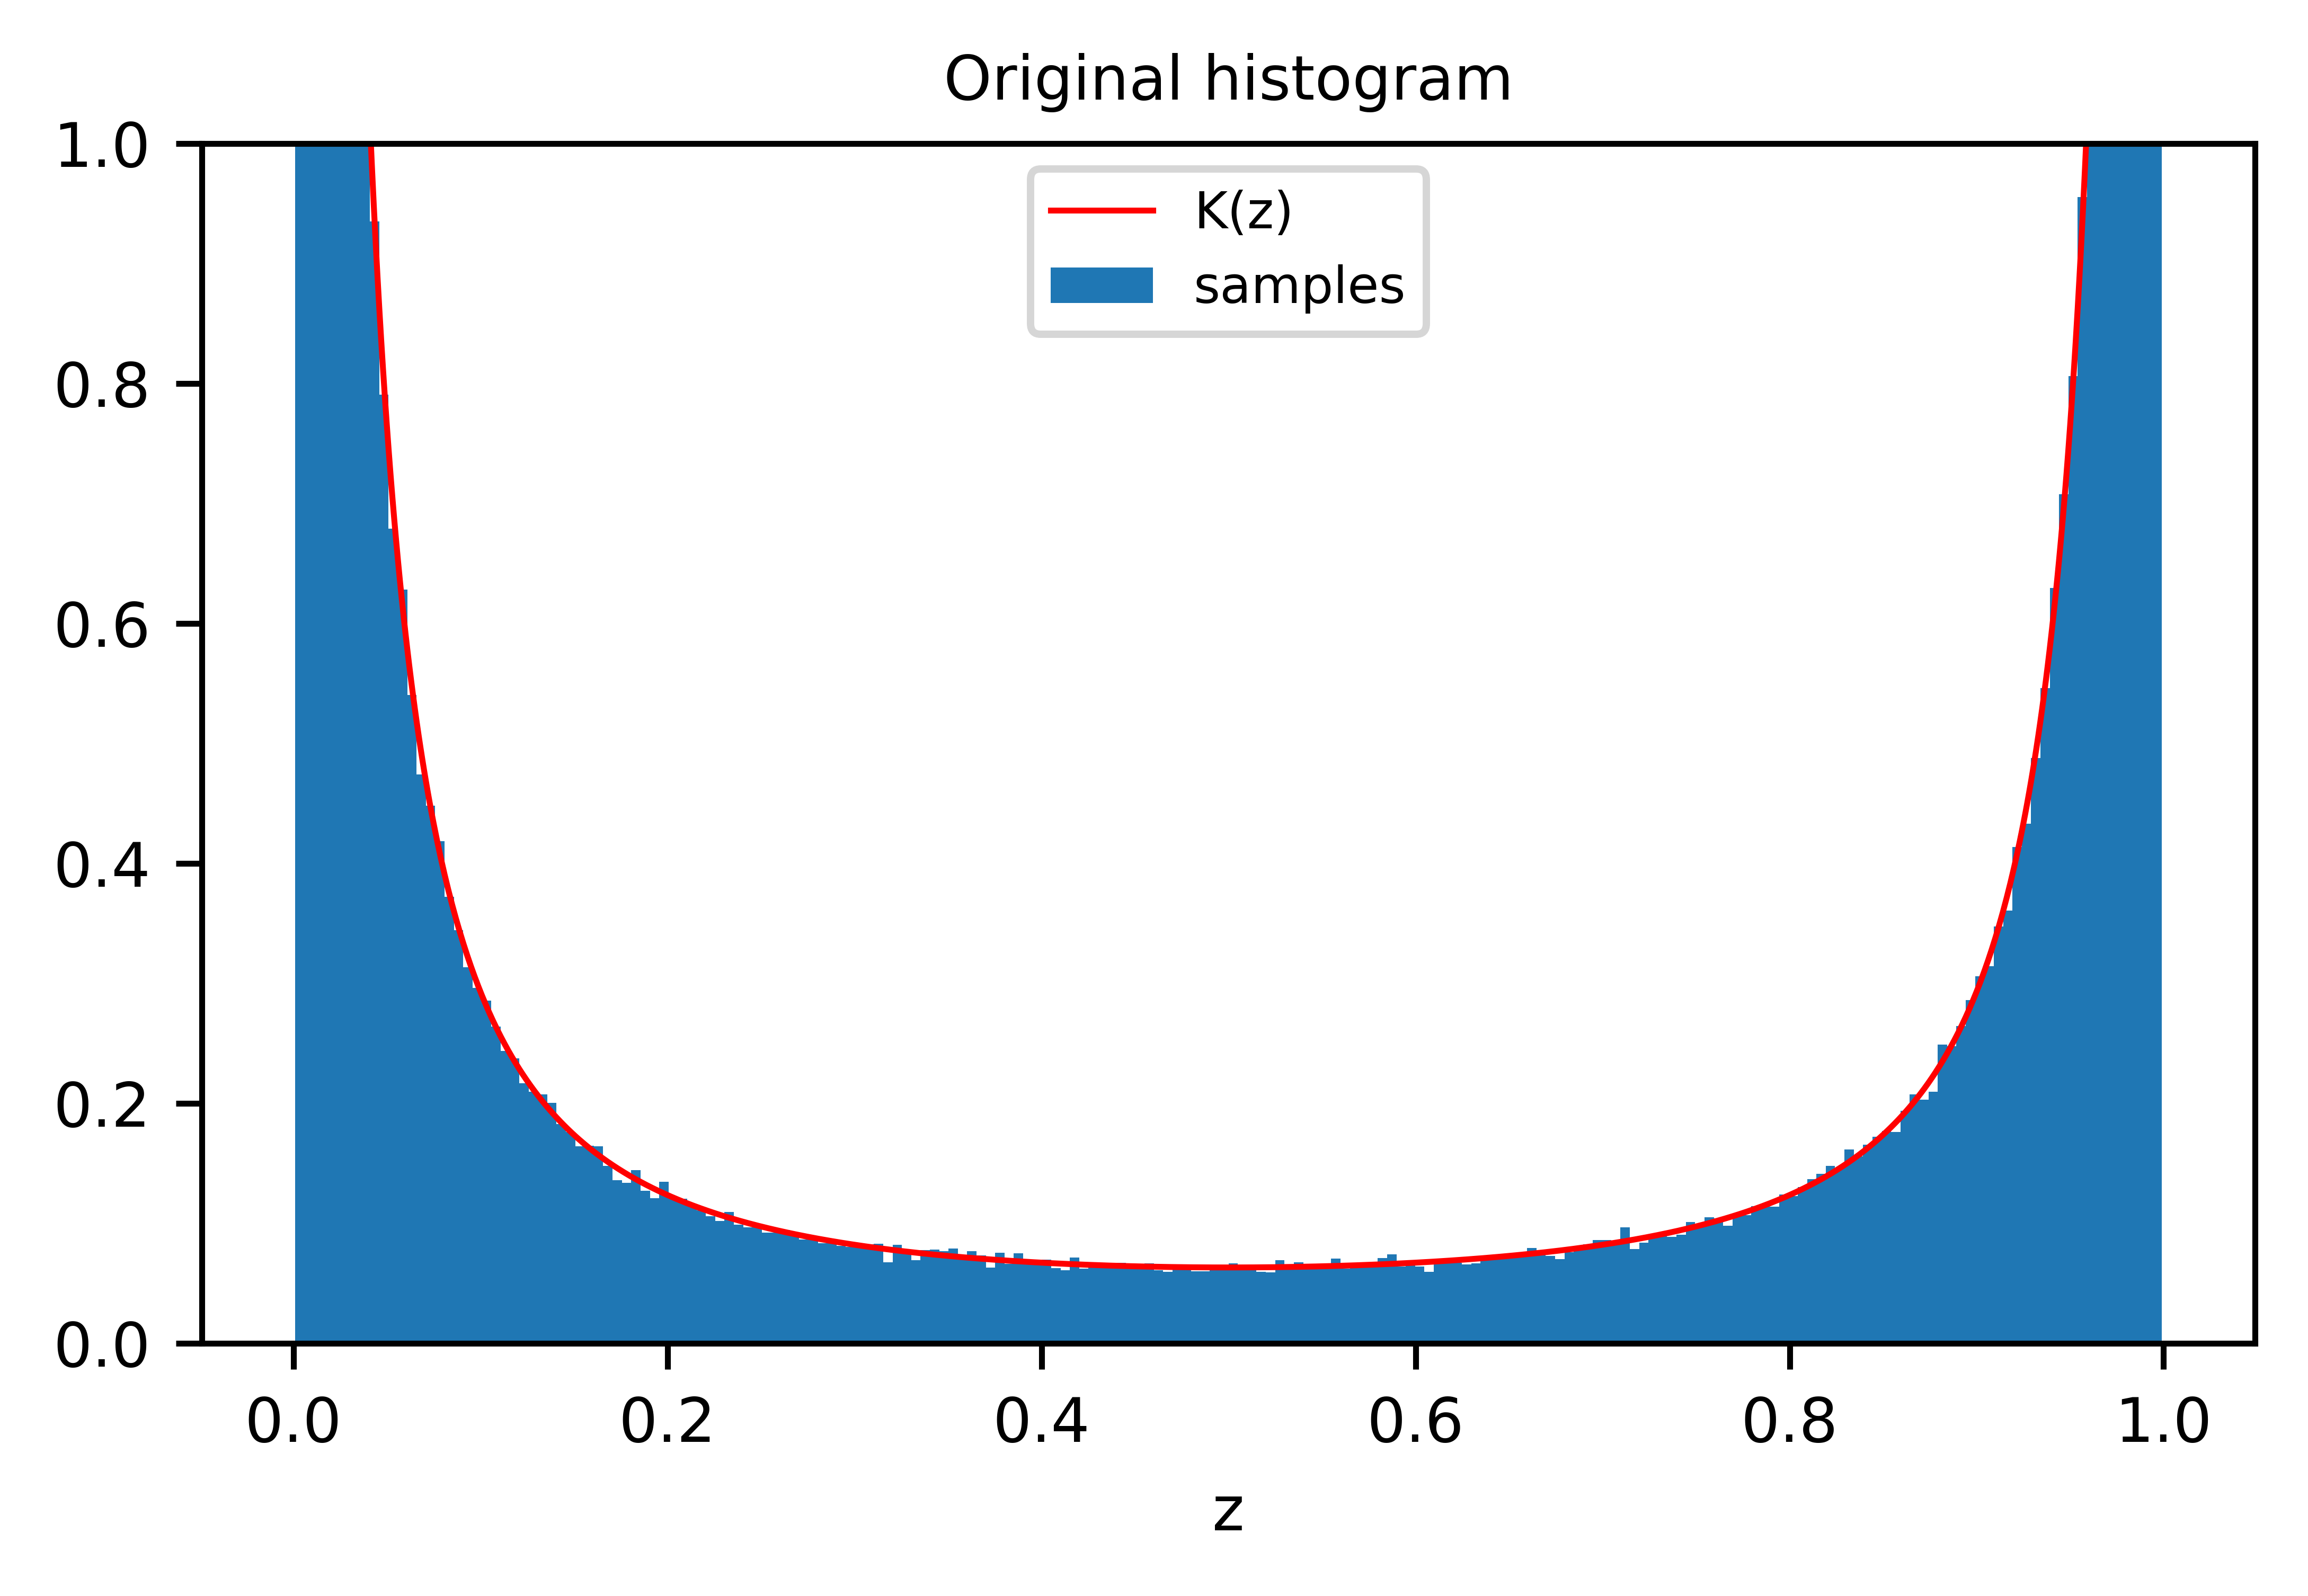
\includegraphics[width=10cm]{pictures/splitting_functions/medium_gg_samples.png}
    \caption{Plot of the simplified kernel \(\mathcal{K}(z)\) for \(gg\) splittings in medium, compared to the sampled values as calculate by \autoref{eqn: medium_gg_sampling}. Total of  \(1,000,000\) samples.}
    \label{fig: medium_gg_sampling}
\end{figure}

\subsection{Monte Carlo implementation}
blah
\subsection{Validating MC results}
blah
\subsubsection{Comparison with analytical results}
Blah

\end{document}